\documentclass[11pt]{article}
\usepackage{amsmath,amssymb}
\usepackage{array}
\usepackage{graphicx}
\usepackage[margin=1.1in]{geometry}
\usepackage{hyperref}

\newcommand{\Fa}{\mathcal{F}_a}
\newcommand{\Fb}{\mathcal{F}_b}
\newcommand{\Fan}{\mathcal{F}_{a,n}}
\newcommand{\Fbn}{\mathcal{F}_{b,n}}

\title{Numerical evaluation, matrix representation,\\
and cascade application of decay feed-down}
\author{Notes accompanying \texttt{DecaySpectra.jl} and
\texttt{CascadeTables.jl}}
\date{\today}

\begin{document}
\maketitle

These notes accompany \texttt{DecaySpectra.jl} and
\texttt{CascadeTables.jl}.  For the decays with two, three, or four daughters
in the main physics notes (whose equation numbers are used below), they
document how each map is (i) reduced to a form that fixed-order
Gauss--Legendre quadrature evaluates rapidly, (ii) precomputed as a matrix
acting on a parent spectrum sampled on a fixed grid, and (iii) composed
through the full resonance cascade.

\paragraph{How to read this.}
The presentation is \emph{topic by topic}, and within each topic the
\emph{analytic} structure is kept separate from its \emph{numerical}
treatment: first what an integral \emph{is} --- its domain, its
singularities, any closed-form structure --- then how it is \emph{computed}.
The topics build on one another:
\begin{itemize}
\item the two-body kernel and its quadrature (Sec.~\ref{sec:quadrature});
\item the effective-mass average that carries three- and four-body decays
(Sec.~\ref{sec:extensions});
\item finite resonance widths (Sec.~\ref{sec:width});
\item the matrix representation for boost-invariant sources
(Sec.~\ref{sec:matrix});
\item full-list table construction, cascade ordering, memory, and persistence
(Sec.~\ref{sec:cascade});
\item its block-Toeplitz generalization to rapidity-dependent sources
(Sec.~\ref{sec:rapidity});
\item the validated numerical domain, regression evidence, and known boundary
cases (Sec.~\ref{sec:validation}).
\end{itemize}
One device recurs throughout and is worth keeping in mind: every multi-body
or finite-width complication is an \emph{average of the same two-body-kernel
implementation} over an effective-mass or spectral distribution.  A
multi-body decay changes only the cheap averaging weight at fixed parent
mass; a finite parent width evaluates that kernel at several parent-mass
nodes and folds the results into one same-shape matrix.

\section{The decay map is linear}

After the analytic azimuthal integration, the daughter spectrum of the
two-body decay $a\to b+c$ is [Eq.~(32)]
\begin{equation}
\Fb(p_T,\eta_p,\phi_p)
 = \frac{B\,m_a}{4\pi\,p^a_{b|c}}
 \int_0^\infty \! q_T\,\mathrm{d}q_T \int_{-\infty}^{\infty}\!\mathrm{d}\eta_q\,
 \frac{\Theta\!\left(Q^2-D^2\right)}{\sqrt{Q^2-D^2}}
 \Big[\Fa(q_T,\eta_q,\phi_p+\alpha)+\Fa(q_T,\eta_q,\phi_p-\alpha)\Big],
 \label{eq:map}
\end{equation}
with $M=m_{aT}m_{bT}$, $Q=q_Tp_T$, $C=m_aE^a_{b|c}$,
$D=M\cosh(\eta_q-\eta_p)-C$, $Z=D/Q$, $\alpha=\arccos Z$.  The three-body
decay [Eq.~(59)] is the same kernel averaged over the effective mass $\mu$
of the $c+d$ pair with weight $p^a_b(\mu)\,p^{\tilde c}_c(\mu)/\mathcal
N_{a\to bcd}$ [Eqs.~(45)--(48)].  In Fourier modes,
$\mathcal F=\sum_n \mathcal F_n e^{in\phi}$ [Eq.~(62)], the two azimuthal
roots produce the Chebyshev factor $2T_n(Z)$ [Eqs.~(40), (41), (61)].

The essential observation is that \eqref{eq:map} is \emph{linear} in
$\Fa$.  Once the parent spectrum is represented by its values on a fixed
grid, the map is a matrix, built once per decay and per mode; applying it
to any source is a matrix--vector product.

\section{The two-body kernel}
\label{sec:quadrature}

Both decays reduce to the double integral
\begin{equation}
K(E_b)=\int q_T\,\mathrm{d}q_T\int\mathrm{d}\eta_q\,
\frac{\Theta\!\left(Q^2-D^2\right)}{\sqrt{Q^2-D^2}}\,
\big[\text{bracket}\big],
\qquad p_b=\sqrt{E_b^2-m_b^2},\quad C=m_aE_b,
\label{eq:K}
\end{equation}
where the bracket is the source sum of \eqref{eq:map} (or $2T_n(Z)\Fan$
in mode form).  The integrand lives on a compact region with
inverse-square-root boundary singularities.  Section~\ref{sec:kernel-analytic}
fixes that region in closed form and locates every non-smooth feature: the
$1/\sqrt{\phantom{x}}$ window edges and a single logarithmic singularity where
the domain changes topology.  Section~\ref{sec:kernel-numeric} removes each by
one substitution, so that plain tensor-product Gauss--Legendre converges
rapidly.

\subsection{Analytic structure: domain and singularities}
\label{sec:kernel-analytic}

\subsubsection{The rapidity-difference window}
\label{sec:window}

\paragraph{What the window is.}
Before the algebra, the physical content.  The analytic azimuthal
integration of the main notes rests on the on-shell $\delta$-function
$\delta(q\cdot p+m_aE_b)$ [Eq.~(4)], which at fixed rapidities fixes the
relative azimuth through $\cos\Delta\phi=Z$ [Eq.~(19)], with
\begin{equation}
Z=\frac{M\cosh\Delta\eta-C}{Q}=\frac{D}{Q}.
\end{equation}
A real opening angle $\Delta\phi$ exists \emph{iff} $|Z|\le1$ [Eq.~(21)]
--- and $\Theta(Q^2-D^2)=\Theta(1-Z^2)$ is exactly the indicator of that
condition.  So the ``$\Delta\eta$ window'' answers a kinematic question:
\emph{for a daughter observed at $(p_T,\eta_p)$, which parent momenta
$(q_T,\eta_q)$ can produce it?}  The parent must sit at a rapidity
separation $\Delta\eta$ for which some azimuthal orientation places the
daughter at $p_T$; too small or too large a $\cosh\Delta\eta$ makes
$|Z|>1$ and no real $\Delta\phi$ exists.  The endpoints $Z=\pm1$ are the
grazing configurations $\Delta\phi=0,\pi$ (daughter emitted parallel or
antiparallel to the parent's transverse momentum), and the
$1/\sqrt{Q^2-D^2}=1/(Q\sqrt{1-Z^2})$ factor is the Jacobian
$|\mathrm{d}\cos\Delta\phi/\mathrm{d}\Delta\phi|^{-1}$ that diverges
integrably there, as at any turning point.

\paragraph{The bounds.}
Throughout, $M=m_{aT}m_{bT}>0$, $Q=q_Tp_T\ge0$ (with $Q>0$ for interior
nodes, $q_T,p_T>0$), and $C=m_aE_b>0$; all three depend on $q_T$ and/or
$p_T$ but not on $\Delta\eta$.  At fixed $q_T$ the integrand is supported
where the argument of the $\Theta$ function is positive:
\begin{equation}
Q^{2}-D^{2}\ge0
\;\iff\;
|D|\le Q
\;\iff\;
-Q\;\le\;M\cosh\Delta\eta-C\;\le\;Q .
\end{equation}
Adding $C$ and dividing by $M>0$ (both operations preserve the
inequalities) gives the two-sided condition
\begin{equation}
\frac{C-Q}{M}\;\le\;\cosh\Delta\eta\;\le\;\frac{C+Q}{M} .
\label{eq:coshwindow}
\end{equation}
This must be intersected with the range of the hyperbolic cosine,
$\cosh\Delta\eta\ge1$.  Two of the three bounds compare trivially:
$(C-Q)/M\le(C+Q)/M$ always (they differ by $2Q/M\ge0$).  Therefore
\begin{equation}
\cosh\Delta\eta\;\in\;
\Big[\max\!\Big(1,\tfrac{C-Q}{M}\Big),\;\tfrac{C+Q}{M}\Big],
\label{eq:coshset}
\end{equation}
and this interval is nonempty \emph{iff} its upper end clears the lower:
since $\max(1,(C-Q)/M)\le(C+Q)/M$ reduces --- whichever branch the max
takes --- to the single condition
\begin{equation}
\frac{C+Q}{M}\;\ge\;1
\;\iff\;
M\;\le\;C+Q ,
\label{eq:nonempty}
\end{equation}
because the branch $(C-Q)/M\le(C+Q)/M$ holds unconditionally.
Condition \eqref{eq:nonempty} is the origin of the $q_T$ band of
Sec.~\ref{sec:band}.

To translate \eqref{eq:coshset} into a set in $\Delta\eta$: on
$\Delta\eta\ge0$ the map $\Delta\eta\mapsto\cosh\Delta\eta$ is strictly
increasing and continuous, so the preimage of the interval
\eqref{eq:coshset} is the interval $[\eta_{\rm lo},\eta_{\rm hi}]$ with
\begin{equation}
\eta_{\rm hi}=\operatorname{arccosh}\frac{C+Q}{M},
\qquad
\eta_{\rm lo}=
\begin{cases}
\operatorname{arccosh}\dfrac{C-Q}{M}, & C-Q>M,\\[4pt]
0, & C-Q\le M ,
\end{cases}
\label{eq:window}
\end{equation}
(the second case includes $C-Q\le0$, where the lower constraint in
\eqref{eq:coshwindow} is vacuous since $\cosh\ge1>\!(C-Q)/M$).  Since
$\cosh$ is even, the full solution set is symmetric,
\begin{equation}
\big\{\Delta\eta:\;|\Delta\eta|\in[\eta_{\rm lo},\eta_{\rm hi}]\big\}
=\big[-\eta_{\rm hi},-\eta_{\rm lo}\big]\cup
 \big[\eta_{\rm lo},\eta_{\rm hi}\big]:
\end{equation}
two disjoint intervals when $\eta_{\rm lo}>0$ (the parent \emph{must} be
at different rapidity than the daughter), merging into the single
interval $[-\eta_{\rm hi},\eta_{\rm hi}]$ when $\eta_{\rm lo}=0$.  The
change between the two topologies as $q_T$ varies is the origin of the
logarithmic singularity of Sec.~\ref{sec:logsing}.

Geometrically the two regimes read as follows.  When $\eta_{\rm lo}>0$
(i.e.\ $C-Q>M$, meaning $C$ is large: the parent is slow or the daughter
hard) the parent cannot sit at the same rapidity as the daughter --- a
co-moving parent would have to emit the daughter with $|Z|>1$ --- so the
allowed set is two rapidity bands straddling $\eta_p$, symmetric about it.
As $q_T$ increases, $Q$ grows, $C-Q$ eventually drops below $M$, the inner
gap closes ($\eta_{\rm lo}\to0$), and the bands merge: now a parent
\emph{at} the daughter's rapidity can feed it (with $\Delta\phi$ given by
the interior value $Z(0)=(M-C)/Q\in(-1,1)$).  The merging point is exactly
$q_T^{*}$ of Sec.~\ref{sec:logsing}.  The upper edge $\eta_{\rm hi}$ always
exists (some maximal rapidity separation beyond which the boost carries the
daughter past $p_T$ for every azimuth) and is always a genuine
$1/\sqrt{\phantom{x}}$ singularity; the lower edge is singular only in the
two-band regime.
Both rapidity signs $\Delta\eta\gtrless0$ contribute; they are evaluated
separately because the source need not be symmetric in rapidity.  At the
window edges $Z=\pm1$ and $Q^2-D^2$ vanishes \emph{linearly} in
$\Delta\eta$: writing $Q^{2}-D^{2}=(Q-D)(Q+D)$ (the factored form is also
what is computed --- it avoids the cancellation of subtracting two large
squares), one factor vanishes at each edge while
$\mathrm{d}D/\mathrm{d}\Delta\eta=M\sinh\Delta\eta\neq0$ there, so the
zero is simple and the integrand diverges as an integrable
$1/\sqrt{\phantom{x}}$.  When $\eta_{\rm lo}=0$ (merged window) the lower
edge is \emph{not} singular --- $Z(0)=(M-C)/Q$ lies inside $(-1,1)$ ---
and the cosine map's clustering there is merely harmless.  Two numerical
guards accompany the window: $q_T$ nodes with $(C+Q)/M\le1$ are skipped
(roundoff can push a node marginally outside the support), and inside the
loop $S_2=(Q-D)(Q+D)\le0$ nodes are dropped for the same reason.

\subsubsection{The transverse-momentum band}
\label{sec:band}

By \eqref{eq:nonempty}, the window is nonempty exactly when
\begin{equation}
m_{aT}\,m_{bT}\;\le\;C+q_Tp_T .
\label{eq:support}
\end{equation}
Both sides of \eqref{eq:support} are strictly positive ($C=m_aE_b>0$ and
$m_{aT}m_{bT}>0$), so squaring preserves the inequality in both
directions and is an equivalence.  Squaring and expanding with
$m_{aT}^2=m_a^2+q_T^2$, $m_{bT}^2=m_b^2+p_T^2$:
\begin{align}
\big(m_a^2+q_T^2\big)\big(m_b^2+p_T^2\big)
&\;\le\; C^2+2Cp_T\,q_T+q_T^2p_T^2 ,\nonumber\\
m_a^2m_b^2+m_a^2p_T^2+m_b^2q_T^2+q_T^2p_T^2
&\;\le\; C^2+2Cp_T\,q_T+q_T^2p_T^2 .
\end{align}
The $q_T^2p_T^2$ terms cancel; using $m_a^2m_b^2+m_a^2p_T^2 =
m_a^2m_{bT}^2$ and collecting powers of $q_T$,
\begin{equation}
m_b^2\,q_T^2-2Cp_T\,q_T+m_a^2m_{bT}^2-C^2\;\le\;0 ,
\label{eq:quadratic}
\end{equation}
a upward parabola in $q_T$: the inequality holds between its roots.  The
quarter-discriminant is
\begin{align}
\tfrac14\Delta
&= (Cp_T)^2-m_b^2\big(m_a^2m_{bT}^2-C^2\big)
 = C^2\big(p_T^2+m_b^2\big)-m_a^2m_b^2\,m_{bT}^2 \nonumber\\
&= m_{bT}^2\big(C^2-m_a^2m_b^2\big)
 = m_{bT}^2\,m_a^2\big(E_b^2-m_b^2\big)
 = m_{bT}^2\,m_a^2\,p_b^2\;\ge\;0 ,
\end{align}
where the second line used $p_T^2+m_b^2=m_{bT}^2$, then $C=m_aE_b$, then
$p_b^2=E_b^2-m_b^2$.  The discriminant is a perfect square --- the roots
are always real, as they must be (the band exists for every open decay).
The quadratic formula then gives
\begin{equation}
q_T^{\pm}
=\frac{Cp_T\pm m_a p_b\,m_{bT}}{m_b^{2}}
=\frac{m_a\big(E_b\,p_T\pm p_b\,m_{bT}\big)}{m_b^{2}},
\qquad
q_T\in\big[\max(0,q_T^-),\,q_T^+\big].
\label{eq:band}
\end{equation}
The sign of the lower root follows from
$\big(E_bp_T\big)^2-\big(p_bm_{bT}\big)^2
= E_b^2p_T^2-p_b^2\big(m_b^2+p_T^2\big)
= p_T^2\big(E_b^2-p_b^2\big)-p_b^2m_b^2
= m_b^2\big(p_T^2-p_b^2\big)$,
so $q_T^->0\iff p_T>p_b$.
The lower root is positive iff $p_T>p_b$: a daughter harder than the
rest-frame momentum can only come from a moving parent, while for
$p_T<p_b$ even a parent at rest contributes and the band starts at
$q_T=0$.

The band width, $q_T^{+}-q_T^{-}=2m_a p_b m_{bT}/m_b^{2}$, carries the
$m_b^{-2}$ of the roots: light daughters have enormous bands
(for $\rho\to\pi\pi$ at $p_T=0.6$\,GeV the band is
$[0.5,\,18]$\,GeV), which is why the feed-down matrices of
Sec.~\ref{sec:matrix} are effectively dense.  In practice the reach in
$q_T$ is limited not by the band but by the source: for a thermal-like
parent spectrum $\sim e^{-(m_{aT}-m_a)/T_{\rm eff}}$ the integrand is
negligible beyond
\begin{equation}
q_T^{\max}\;=\;\sqrt{\big(m_a+T_{\rm eff}\ln(1/\varepsilon)\big)^{2}-m_a^{2}},
\label{eq:qtmax}
\end{equation}
($\varepsilon$ the tolerated relative tail, e.g.\ $10^{-8}$), which also
sets the required extent of any fixed parent grid.  Note that
$T_{\rm eff}$ is the slope of the \emph{actual} source --- radial flow
blueshifts it well above the freeze-out temperature.

\subsubsection{The logarithmic singularity at the internal band point}
\label{sec:logsing}

Inside the band the window changes topology where $\eta_{\rm lo}$ reaches
zero, i.e.\ where $C-Q-M$ changes sign (case boundary of
\eqref{eq:window}).  Solving $m_{aT}m_{bT}=C-q_Tp_T$ by the same
squaring as in Sec.~\ref{sec:band} --- legitimate on the branch
$C-q_Tp_T\ge0$, which holds there since $m_{aT}m_{bT}>0$ --- flips only
the sign of the linear term in \eqref{eq:quadratic}, so the roots are
$-q_T^{\mp}$, and the positive one is
\begin{equation}
q_T^{*}=\frac{m_a\big(p_b\,m_{bT}-E_b\,p_T\big)}{m_b^{2}}=-\,q_T^- ,
\end{equation}
which lies inside the band $(0,q_T^{+})$ precisely when $q_T^-<0$, i.e.\
$p_T<p_b$.

For the local behavior define $g\equiv Q+M-C$, so $g<0$ is the
two-interval regime ($\eta_{\rm lo}>0$) and $g>0$ the merged one, with
$g(q_T^{*})=0$; $g$ is strictly increasing in $q_T$
($\mathrm{d}g/\mathrm{d}q_T = p_T + q_T\,m_{bT}/m_{aT}>0$), so near the
transition $g\simeq g'(q_T^{*})\,(q_T-q_T^{*})$.  Expand the integrand
factors around $\Delta\eta=0$ using
$\cosh\Delta\eta=1+\tfrac12\Delta\eta^{2}+\mathcal O(\Delta\eta^{4})$:
\begin{equation}
Q+D=Q+M\cosh\Delta\eta-C
 \;=\; g+\tfrac12 M\Delta\eta^{2}+\mathcal O(\Delta\eta^{4}),
\qquad
Q-D\;=\;2Q-g-\tfrac12M\Delta\eta^{2}\;\simeq\;2Q ,
\end{equation}
the second factor staying regular (it vanishes at the \emph{other} edge
$\eta_{\rm hi}$, far from $\Delta\eta=0$).  Hence, up to a cutoff
$\Lambda$ separating the local region from the rest of the window,
\begin{equation}
\int\frac{\mathrm{d}\Delta\eta}{\sqrt{(Q-D)(Q+D)}}
\;\simeq\;
\frac{1}{\sqrt{2Q}}\int\frac{\mathrm{d}\Delta\eta}
{\sqrt{g+\tfrac12M\Delta\eta^{2}}} ,
\end{equation}
and the local integral has elementary antiderivatives on both sides of
the transition:
\begin{align}
g>0:&\quad
\int_{0}^{\Lambda}\frac{\mathrm{d}\Delta\eta}
{\sqrt{g+\tfrac12M\Delta\eta^{2}}}
=\sqrt{\tfrac{2}{M}}\,
\operatorname{arcsinh}\!\Big(\Lambda\sqrt{\tfrac{M}{2g}}\Big)
=\sqrt{\tfrac{2}{M}}\Big[\ln\!\big(2\Lambda\sqrt{\tfrac{M}{2}}\big)
-\tfrac12\ln g\Big]+\mathcal O(g),\\
g<0:&\quad
\int_{\eta_{\rm lo}}^{\Lambda}\frac{\mathrm{d}\Delta\eta}
{\sqrt{\tfrac12M\big(\Delta\eta^{2}-\eta_{\rm lo}^{2}\big)}}
=\sqrt{\tfrac{2}{M}}\,
\operatorname{arccosh}\!\Big(\frac{\Lambda}{\eta_{\rm lo}}\Big)
=\sqrt{\tfrac{2}{M}}\Big[\ln\!\big(2\Lambda\sqrt{\tfrac{M}{2}}\big)
-\tfrac12\ln|g|\Big]+\mathcal O(g),
\end{align}
where the second line used $g+\tfrac12M\Delta\eta^{2}
=\tfrac12M(\Delta\eta^{2}-\eta_{\rm lo}^{2})$ with
$\eta_{\rm lo}=\sqrt{-2g/M}$ and
$\operatorname{arccosh}x=\ln(2x)+\mathcal O(x^{-2})$.  Both sides carry
the \emph{same} coefficient $-\tfrac12\sqrt{2/M}\,\ln|g|$: the inner
integral has a symmetric, integrable logarithmic singularity
\begin{equation}
I(q_T)\;=\;-\frac{1}{\sqrt{2QM}}\,\ln\big|q_T-q_T^{*}\big|
\;+\;\text{(regular)} ,
\label{eq:logsing-form}
\end{equation}
after inserting the linearization of $g$.  A Gauss rule straddling a
logarithm converges only algebraically, so the $q_T$ interval is split at
$q_T^{*}$ whenever $q_T^-<0<q_T^{*}<q_T^+$; the residual
$\theta\ln\theta$ endpoint behavior after the cosine map is discussed in
Sec.~\ref{sec:cosmap}.

\subsection{Numerical treatment: the cosine-mapped Gauss rule}
\label{sec:kernel-numeric}

Every non-smooth feature located above is removed by a single substitution:
the $1/\sqrt{\phantom{x}}$ window edges and the $\sqrt{\phantom{x}}$ zeros of
the $\mu$ average both cancel against a cosine map's Jacobian, leaving the
lone $q_T^{*}$ logarithm, which is isolated by splitting the interval there.

\subsubsection{The cosine substitution and the tensor-product rule}
\label{sec:cosmap}

Every one-dimensional interval $[x_{\rm lo},x_{\rm hi}]$, of midpoint
$m=\tfrac12(x_{\rm lo}+x_{\rm hi})$ and half-width
$h=\tfrac12(x_{\rm hi}-x_{\rm lo})$, is traversed via
\begin{equation}
x(\theta)=m-h\cos\theta,
\qquad \theta\in(0,\pi),
\qquad
\mathrm{d}x=h\,\sin\theta\,\mathrm{d}\theta ,
\label{eq:cosmap}
\end{equation}
which maps $\theta=0\mapsto x_{\rm lo}$ and $\theta=\pi\mapsto
x_{\rm hi}$ monotonically.  The endpoint expansion is exact in
half-angle form:
\begin{equation}
x-x_{\rm lo}=h\,(1-\cos\theta)=2h\sin^{2}\tfrac{\theta}{2},
\qquad
x_{\rm hi}-x=h\,(1+\cos\theta)=2h\cos^{2}\tfrac{\theta}{2}.
\label{eq:halfangle}
\end{equation}
Consider an integrand with the inverse-square-root endpoint behavior
established in Sec.~\ref{sec:window},
$f(x)=g(x)/\sqrt{(x-x_{\rm lo})(x_{\rm hi}-x)}$ with $g$ smooth.  Using
\eqref{eq:halfangle} and $\sin\theta=2\sin\tfrac\theta2\cos\tfrac\theta2$,
\begin{equation}
f\big(x(\theta)\big)\,\frac{\mathrm{d}x}{\mathrm{d}\theta}
=\frac{g\big(x(\theta)\big)\; h\cdot2\sin\tfrac\theta2\cos\tfrac\theta2}
{\sqrt{2h\sin^{2}\tfrac\theta2\;\cdot\;2h\cos^{2}\tfrac\theta2}}
=g\big(x(\theta)\big):
\label{eq:cancel}
\end{equation}
the singular factors cancel \emph{identically}, not just to leading
order --- the $\theta$-integrand is as smooth as $g$, and Gauss--Legendre
in $\theta$ converges spectrally.  (If only one endpoint is singular the
cancellation happens there and the other endpoint merely gains harmless
node clustering; endpoint zeros $\propto\sqrt{x-x_{\rm lo}}$, as in the
$\mu$ integral, become smooth $\propto\sin^{2}\tfrac\theta2$ by the same
algebra.)

The $\theta$ integral itself is discretized by an $n$-point
Gauss--Legendre rule with nodes $x_i\in(-1,1)$ and weights $w_i$, mapped
affinely to $(0,\pi)$: $\theta_i=\tfrac\pi2(x_i+1)$,
$\int_0^\pi G\,\mathrm{d}\theta\approx\tfrac\pi2\sum_iw_iG(\theta_i)$.
Combining with \eqref{eq:cosmap},
\begin{equation}
\int_{x_{\rm lo}}^{x_{\rm hi}}f(x)\,\mathrm{d}x
\;\approx\;
h\sum_{i=1}^{n} v_i\, f\big(m-h\,c_i\big),
\qquad
c_i=\cos\theta_i,\quad
v_i=\tfrac{\pi}{2}\,w_i\sin\theta_i ,
\label{eq:fusedweights}
\end{equation}
so the map costs no trigonometry at evaluation time: the fused pairs
$(c_i,v_i)$ are computed once per order and shared (memoized) across all
decay objects.  Applying \eqref{eq:fusedweights} in both directions gives
the tensor-product kernel sum
\begin{equation}
K(E_b)\;\approx\;
\sum_{\text{seg}}\;h_q\sum_{i=1}^{n_q} v^{q}_{i}\;q_T^{(i)}\;
h_\eta\!\left(q_T^{(i)}\right)\sum_{j=1}^{n_\theta} \frac{v^{\theta}_{j}}
{\sqrt{Q^{2}-D_{ij}^{2}}}\,\big[\text{bracket}\big]_{ij},
\label{eq:tensor}
\end{equation}
where the inner $1/\sqrt{\phantom{x}}$ is evaluated in the factored form
$(Q-D)(Q+D)$ and the singular endpoint behavior is tamed by
\eqref{eq:cancel} through the mapped $\Delta\eta$ nodes.  The only
residual non-smoothness is the logarithm of Sec.~\ref{sec:logsing} at the
segment endpoint $q_T^{*}$: with $x-q_T^{*}\propto\theta^{2}$ from
\eqref{eq:halfangle}, the integrand behaves as
$\sin\theta\cdot\ln\theta^{2}\sim2\,\theta\ln\theta$ near $\theta=0$ ---
continuous but not analytic --- for which the Gauss error decreases
algebraically, $\sim n_q^{-4}$ (measured: the error at low $p_T$ drops
$\approx16\times$ per doubling of $n_q$).

\subsubsection{The two regimes, and what the split is worth}
\label{sec:segment-figure}

Figure~\ref{fig:nodes} shows the object being integrated, for
$\rho\to\pi\pi$ with a static thermal source.  Which regime applies is decided
by a single comparison.  The split point $q_T^{*}=-q_T^{-}$ lies inside the
band $(0,q_T^{+})$ only when $q_T^{-}<0$, i.e.\ when $p_T<p_b$, the daughter's
rest-frame momentum: a daughter slower than $p_b$ can be emitted both forward
and backward into the same laboratory $p_T$, and $q_T^{*}$ is where those two
branches meet.  For $\rho\to\pi\pi$, $p_b=0.362$~GeV, so the split is needed
throughout the soft region that dominates the yield and is absent above it.

In the left panel ($p_T=0.15$~GeV) the logarithm of \eqref{eq:logsing-form}
is plainly visible at $q_T^{*}=0.635$~GeV.  A single Gauss segment spanning
the whole band (circles) places its nodes by the cosine map of
\eqref{eq:cosmap}, which clusters them at the band \emph{edges} --- exactly
where the integrand is featureless --- and straddles the spike with a handful
of widely spaced points.  Splitting at $q_T^{*}$ (triangles) makes the
singular point an endpoint of both segments, so the same clustering that was
wasted on the edges now resolves the logarithm from either side.  In the right
panel ($p_T=0.80$~GeV) the singularity has left the band, the integrand is
smooth on $(q_T^{-},q_T^{+})$, and one segment is enough.

The third panel measures the difference at $p_T=0.15$~GeV against a converged
reference.  Splitting recovers the predicted $n_q^{-4}$ of the residual
$\theta\ln\theta$ endpoint; the unsplit rule, with an interior logarithm,
decays as $n_q^{-0.8}$ and is still at the percent level with $n_q=256$.  At
the production order $n_q=128$ the split rule is accurate to $7\times10^{-8}$
and the unsplit one to $2\times10^{-2}$ --- a factor of $3\times10^{5}$ for a
branch and one extra segment loop.

\begin{figure}[htbp]
\centering
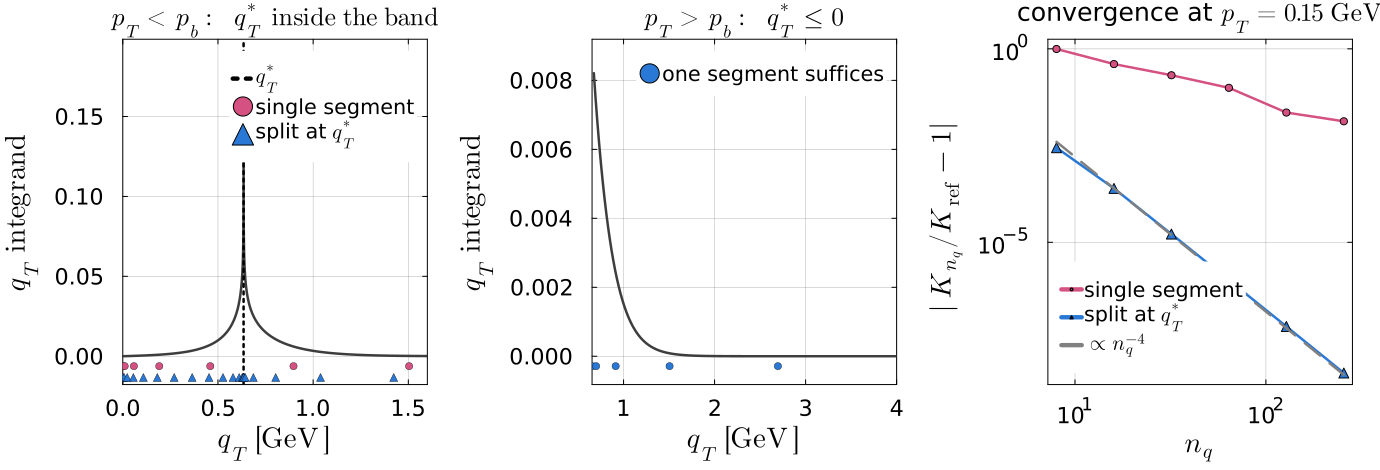
\includegraphics[width=\linewidth]{figures/quadrature_nodes.png}
\caption{The $q_T$ integrand of \eqref{eq:tensor} for $\rho\to\pi\pi$ with a
static thermal source at $T=0.155$~GeV, and the $n_q=16$ node positions the
cosine-mapped rule assigns to it.  \emph{Left:} $p_T=0.15\,\mathrm{GeV}<p_b$,
so $q_T^{*}$ (dotted) lies inside the band and carries the logarithm of
\eqref{eq:logsing-form}; nodes are shown for a single segment (circles) and
for the split at $q_T^{*}$ (triangles).  \emph{Right:}
$p_T=0.80\,\mathrm{GeV}>p_b$, where $q_T^{*}\le0$, the integrand is smooth,
and one segment suffices.  Both bands extend well beyond the plotted range
($q_T^{+}=5.3$ and $24.0$~GeV respectively) into the exponentially suppressed
tail, where the remaining nodes lie.  \emph{Far right:} relative error of the
kernel against a converged reference at $p_T=0.15$~GeV.  Generated by
\texttt{figures/quadrature\_nodes.jl}.}
\label{fig:nodes}
\end{figure}

\subsubsection{Three-body: the effective-mass average}

For $a\to b+c+d$ the kernel is averaged over the effective mass
$\mu\in[m_c+m_d,\,m_a-m_b]$ with weight
$p^{\tilde c}_c(\mu)$ and normalization
$\mathcal N=\int\mathrm{d}\mu\,p^a_b(\mu)\,p^{\tilde c}_c(\mu)$
[Eqs.~(45)--(48)].  The integrand vanishes as a square root at both
endpoints: $p^{\tilde c}_c\sim\sqrt{\mu-(m_c+m_d)}$ at threshold, and
$K\propto$ band width $\propto p^a_b(\mu)\sim\sqrt{m_a-m_b-\mu}$ at the
upper limit.  The same substitution \eqref{eq:cosmap} turns
$\sqrt{\phantom{x}}$-type zeros into smooth $\theta^{2}$ behavior, and the
$\mu$ integral is done with an $n_\mu$-point cosine-mapped Gauss rule; the
nodes $\mu_i$, energies $E_b(\mu_i)$ and normalized weights are
precomputed at construction.

\subsubsection{Measured convergence and default orders}

For a Boltzmann source ($T=0.15$\,GeV) relative errors against
high-order references behave as follows (worst case is low $p_T$, where
the $q_T^{*}$ logarithm is inside the band):
\begin{center}
\begin{tabular}{lcc}
\hline
orders & error at $p_T=0.2$ & error at $p_T=0.8$ \\
\hline
$\rho\to\pi\pi$:\; $(n_q,n_\theta)=(128,32)$ & $7\cdot10^{-8}$ & $5\cdot10^{-12}$\\
\phantom{$\rho\to\pi\pi$:}\; $(64,16)$ & $2\cdot10^{-6}$ & $5\cdot10^{-12}$\\
\phantom{$\rho\to\pi\pi$:}\; $(32,8)$ & $3\cdot10^{-6}$ & $2\cdot10^{-8}$\\
\hline
$\omega\to3\pi$:\; $(n_\mu,n_q,n_\theta)=(32,128,32)$ & $2\cdot10^{-8}$ & $3\cdot10^{-13}$\\
\phantom{$\omega\to3\pi$:}\; $(16,64,16)$ & $5\cdot10^{-7}$ & $3\cdot10^{-10}$\\
\phantom{$\omega\to3\pi$:}\; $(8,32,8)$ & $1\cdot10^{-4}$ & $5\cdot10^{-5}$\\
\hline
\end{tabular}
\end{center}
The $\Delta\eta$ direction is spectrally convergent and over-resolved
already at $n_\theta=16$; $n_q$ is limited by the logarithm
($\sim n_q^{-4}$, only relevant for $p_T<p_b$); $n_\mu\ge16$ is safe while
$n_\mu=4$ fails at the percent level.  The exported functor constructors
default to $(n_q,n_\theta,n_\mu)=(128,32,32)$; these settings are
conservative, and cost scales linearly in each order.  The production
\texttt{CascadeTable} instead defaults to
$(n_q,n_\theta,n_\mu,n_\sigma,n_{m_a})=(32,8,8,8,8)$, trading some build
accuracy for speed on its sampled grid.  The continuous-functor regression
tests give number conservation, $N_b=B\,N_a$, at the $10^{-4}$ level or
better, but they use the higher exported-functor defaults; they do not by
themselves certify the production table orders.

\section{Multi-body decays: the effective-mass average}
\label{sec:extensions}

The three-body $\mu$ average of Sec.~\ref{sec:quadrature} is the first
instance of a general pattern: any number of unobserved daughters can be
clustered into a single effective particle of mass $\mu$, and the same
two-body kernel is averaged over that cluster's mass.  This section makes the
pattern explicit --- its \emph{analytic} form is a phase-space recursion, its
\emph{numerical} cost is one extra mass quadrature per additional daughter
--- and applies it to four-body decays.  (Finite widths,
Sec.~\ref{sec:width}, are the very same construction with a spectral function
in place of the phase-space weight.)  Throughout, the question is whether an
extra integration multiplies the \emph{expensive} kernel evaluations or only
enriches the \emph{cheap} weight.

\subsection{Recursive effective-mass structure}
\label{sec:recursive}

Return to the three-body average and read it structurally.  For
$a\to b+(cd)$ the observed daughter $b$ recoils against the pair treated
as a single effective particle $\widetilde{cd}$ of mass $\mu$; the
\emph{angular} distribution of $b$ --- hence the entire $(q_T,\Delta\eta)$
kernel --- depends on the pair only through $\mu$, via
$E_b(\mu)=(m_a^2+m_b^2-\mu^2)/2m_a$.  The internal breakup of the pair
enters solely through \emph{how much probability sits at each} $\mu$,
i.e.\ the invariant-mass density of the pair,
\begin{equation}
\rho_2(\mu;m_c,m_d)\;\propto\;q(\mu;m_c,m_d),
\qquad
q(M;m_1,m_2)\equiv\frac{\lambda^{1/2}(M^2,m_1^2,m_2^2)}{2M},
\end{equation}
which is precisely the weight $p^{\tilde c}_c(\mu)$ of Eq.~(47).  Writing
the map this way,
\begin{equation}
\Fb=\frac{B\,m_a}{4\pi\,\mathcal N}
\int_{\mu_-}^{\mu_+}\!\mathrm{d}\mu\;
\underbrace{p^a_b(\mu)\,\rho_2(\mu)}_{\text{weight}}\;
K\big(E_b(\mu)\big),
\qquad
\mathcal N=\int\mathrm{d}\mu\,p^a_b(\mu)\,\rho_2(\mu),
\label{eq:threebody-recursive}
\end{equation}
makes the generalization immediate.  For an $n$-body decay
$a\to b+(c_1\cdots c_{n-1})$, cluster the $n-1$ unobserved particles into
$\widetilde{c}$ of mass $\mu\in[\sum_i m_{c_i},\,m_a-m_b]$; the kernel is
unchanged, $K(E_b(\mu))$, and only the weight generalizes to the
invariant-mass density $\rho_{n-1}(\mu)$ of the cluster.

\paragraph{Where the density comes from.}
The density and its recursion are the standard factorization of $n$-body
Lorentz-invariant phase space.  Peeling the observed particle $b$ against
the cluster of invariant mass $\mu$,
\begin{equation}
\mathrm{d}\Phi_n\big(m_a^2;\,p_b,\{p_{c_i}\}\big)
=\frac{\mathrm{d}\mu^2}{2\pi}\;
\mathrm{d}\Phi_2\big(m_a^2;\,m_b^2,\mu^2\big)\;
\mathrm{d}\Phi_{n-1}\big(\mu^2;\,\{p_{c_i}\}\big),
\label{eq:phasespace-fact}
\end{equation}
and integrating the two-body factor over the isotropic emission angle,
$\int\mathrm{d}\Phi_2(m_a^2;m_b^2,\mu^2)\propto q(m_a;m_b,\mu)=p^a_b(\mu)$,
identifies the $\mu$-measure as $p^a_b(\mu)\,\mathrm{d}\mu$ times the
cluster's own phase-space volume.  Defining that volume as the density,
$\rho_{n-1}(\mu)\,\mathrm{d}\mu\equiv\int\mathrm{d}\Phi_{n-1}(\mu^2;\{p_{c_i}\})$
at fixed cluster mass, and applying \eqref{eq:phasespace-fact} once more to
$\mathrm{d}\Phi_{n-1}$ --- peeling $c_1$ against the sub-cluster of mass
$\sigma$ --- gives the Byckling--Kajantie recursion, one particle at a time,
\begin{equation}
\rho_{k}\big(\mu;m_{c_1},\dots,m_{c_k}\big)
=\int_{\sigma_-}^{\sigma_+}\!\mathrm{d}\sigma\;
q(\mu;m_{c_1},\sigma)\;\rho_{k-1}\big(\sigma;m_{c_2},\dots,m_{c_k}\big),
\qquad
\rho_1(\sigma;m)=\delta(\sigma-m),
\label{eq:phasespace-recursion}
\end{equation}
with $\sigma\in[\sum_{i\ge2}m_{c_i},\,\mu-m_{c_1}]$.  The overall constants
($2\pi$ from \eqref{eq:phasespace-fact}, the $4\pi$ from each angular
integration) are $\mu$-independent and cancel in the normalized ratio
$\Fb$, so they are dropped.  The recursion terminates at $\rho_1=\delta$ (a
single particle has definite mass); one step gives $\rho_2=q$ (the
three-body weight of Eq.~47), and for four-body
\begin{equation}
\rho_3(\mu;m_c,m_d,m_e)
=\int_{m_d+m_e}^{\mu-m_c}\!\mathrm{d}\sigma\;
q(\mu;m_c,\sigma)\;q(\sigma;m_d,m_e).
\label{eq:rho3}
\end{equation}

\paragraph{The four-body map explicitly.}
Assembling the pieces, the observed-$b$ spectrum of $a\to b\,c\,d\,e$ is the
two-dimensional mass average
\begin{equation}
\begin{aligned}
\Fb
&=\frac{B\,m_a}{4\pi\,\mathcal N}
\int_{m_c+m_d+m_e}^{m_a-m_b}\!\!\mathrm{d}\mu\;p^a_b(\mu)\\
&\quad{}\times
\underbrace{\left[\int_{m_d+m_e}^{\mu-m_c}\!\!\mathrm{d}\sigma\;
q(\mu;m_c,\sigma)\,q(\sigma;m_d,m_e)\right]}_{\rho_3(\mu)}
K\big(E_b(\mu)\big),\\
\mathcal N
&=\int\!\mathrm{d}\mu\,p^a_b(\mu)\rho_3(\mu).
\end{aligned}
\label{eq:fourbody}
\end{equation}
The bracket is the Lorentz-invariant phase-space volume of the
three-particle cluster $c\,d\,e$ at total mass $\mu$ --- geometrically, the
area of its Dalitz plot.  The inner $\sigma$ integral runs over the $(de)$
sub-mass; by the symmetry of phase space any pairing gives the same
$\rho_3$, so the choice of which particle to peel first is free.  Both mass
integrals carry the $\sqrt{\phantom{x}}$-type endpoint zeros of the Källén
function (each $q$ vanishes at its threshold), regularized by the cosine
map of Sec.~\ref{sec:cosmap}.

\paragraph{Cost.}
The crucial point is that $\rho_{n-1}(\mu)$ is \emph{independent of the
kernel}: it is a static, $(n-2)$-fold nested phase-space integral in the
mass variables alone, computed once on the $n_\mu$ nodes at construction.
The number of expensive kernel evaluations therefore stays $n_\mu$ ---
the \emph{same} as three-body --- for any number of unobserved daughters;
only the weight becomes a nested, kernel-free integral.  With $n_\sigma$
points per level that weight costs $n_\mu\,n_\sigma^{\,n-2}$ evaluations of
the elementary function $q$ --- arithmetic only --- against the fixed $n_\mu$
kernel evaluations.  So the build cost is dominated by the kernel until $n$
is large, and a four- or five-body matrix is, in practice, a three-body
matrix with a slightly richer weight.

\paragraph{On observing a cluster particle.}
In the cascade every daughter is observed in turn (Sec.~\ref{sec:matrix}).
When the observed particle is one of the ``cluster'' members, one simply
relabels: the observed particle plays the role of $b$ and the remaining
$n-1$ form the cluster.  The construction above is symmetric under that
relabelling, so nothing new is required --- the observed slot is chosen,
the rest are clustered, and $\rho_{n-1}$ is built from their masses.

\section{Finite widths}
\label{sec:width}

So far every mass has been sharp.  A resonance of width $\Gamma_i$ is
instead spread over a spectral function --- a relativistic Breit--Wigner,
\begin{equation}
\varrho_i(m)\;\propto\;
\frac{m^2\,\Gamma_i(m)}
{\big(m^2-m_i^2\big)^2+m_i^2\,\Gamma_i(m)^2},
\qquad
\int\varrho_i(m)\,\mathrm{d}m=1,
\end{equation}
whose width is itself mass dependent when the resonance decays to two
particles in relative angular momentum $\ell$,
\begin{equation}
\Gamma_i(m)=\Gamma_i\,\frac{m_i}{m}
\left(\frac{q(m;m_1,m_2)}{q(m_i;m_1,m_2)}\right)^{2\ell+1}
\frac{B_\ell\big(q(m)\big)}{B_\ell\big(q(m_i)\big)}
\label{eq:massdep-width}
\end{equation}
($B_\ell$ the Blatt--Weisskopf barrier factor).  It vanishes at threshold
$m=m_1+m_2$, so $\varrho_i$ carries no weight below threshold, and
$\varrho_i\to\delta(m-m_i)$ as $\Gamma_i\to0$.

Equations above describe the general mass-dependent-width construction.
Both specializations are implemented, as subtypes of
\texttt{SpectralShape}, and selected by the \texttt{spectral} table option
(\texttt{CascadeTable}) or the \texttt{shape} keyword
(\texttt{ThermalModel}).  Each returns an \emph{unnormalized} shape on a
caller-specified window; \texttt{BroadParent} normalizes when forming the
parent-mass average.

\texttt{MassDependentBW} is the default.  It implements
\eqref{eq:massdep-width} at $\ell=0$ and \emph{without} the Blatt--Weisskopf
factor, with the symmetric split $q(m)=\sqrt{m^{2}-m_{\rm th}^{2}}/2$, where
$m_{\rm th}$ is the summed daughter mass of the resonance's \emph{lightest}
channel --- so the shape is a property of the species, while each individual
channel's closure remains handled by dropping parent-mass nodes below its own
threshold.  The split is exact for $\sigma\to\pi\pi$ and approximates the
$q$-ratio for asymmetric pairs.  Since $\Gamma(m)$ vanishes at $m_{\rm th}$,
the shape carries no weight where the state cannot decay; for the $\sigma$
that removes the $2.56\%$ of constant-width weight below $2m_\pi$.  A
resonance whose pole lies at or below its own threshold has no $q(m_i)$ and
falls back to the constant shape.

\texttt{BreitWigner} is the constant-width specialization
$\Gamma_i(m)=\Gamma_i$, retained both as that fallback and as the
\texttt{:constant} option.  Barrier factors and per-channel $\ell$ remain
unimplemented.

\paragraph{One principle, two costs.}
Whether a given width is cheap or expensive to include is decided by
\emph{how that mass enters the decay map}.  A mass that enters \emph{only
through the effective cluster mass $\mu$} --- any of the unobserved
daughters --- reshapes the precomputed weight $\rho_{n-1}(\mu)$ and nothing
else, so it costs nothing extra.  A mass that enters the \emph{kinematics of
the observed leg} --- the parent (through $C=m_aE_b$ and the $q_T$ band) or
the observed daughter (through $E_b,p_b$) --- changes the kernel itself, and
must be handled by an \emph{outer average}: one kernel build per mass node.
The three places a width can sit map onto exactly this split:
\begin{itemize}
\item \textbf{Unobserved / cluster masses --- cheap.}  A width on any $c_i$
just averages the sharp momentum inside the phase-space recursion
\eqref{eq:phasespace-recursion},
$q(\mu;m_{c_1},\sigma)\to\int\mathrm{d}m_{c_1}\,\varrho(m_{c_1})\,q(\mu;m_{c_1},\sigma)$.
It modifies $\rho_{n-1}(\mu)$ and touches no kernel.
\item \textbf{Observed daughter $b$ --- expensive, but usually moot.}
$K\to\int\mathrm{d}m_b\,\varrho_b(m_b)\,K$.  The measured $\pi,K,p,\Lambda$
are stable or narrow, so this collapses to the sharp $\delta$; it only
matters for a broad observed resonance mid-cascade.
\item \textbf{Parent $a$ --- expensive, and dominant.}
$\int\mathrm{d}m_a\,\varrho_a(m_a)\,(\cdots)$.  The broadest states
($\sigma,\rho,\Delta,\dots$) are parents, so this is where finite width
matters most.
\end{itemize}

\paragraph{Which case this cascade needs.}
The split above is general, but the cascade of Sec.~\ref{sec:cascade} decays
every resonance in \emph{its own} feeder-before-fed step (mass-descending for
an ordinary pole-open graph): $a\to bR$ and $R\to cc'$ are two separate
two-body decays, never collapsed into one three-body $a\to bcc'$.  A broad
$R$ therefore enters \emph{as a parent} --- when $R$ itself decays --- not as
a cluster mass.  The genuine multi-body channels treated by the
effective-mass integral ($\omega\to3\pi$, $\eta\to3\pi$) have \emph{stable}
daughters, carrying no cluster width either.  The parent average --- the
expensive case --- is thus the main use of the per-species widths, and the
cheap case is kept for completeness.  The next two subsections treat each in
turn.

\subsection{The cheap case: width reweights the effective-mass integral}

Case~1 is not a new mechanism --- it \emph{is} the effective-mass integral
of Sec.~\ref{sec:recursive}.  When the unobserved pair $c\,c'$ forms a
resonance $R$, its density $\rho_2(\mu)=q(\mu;m_c,m_{c'})$ picks up the $R$
propagator and \emph{becomes} a Breit--Wigner peak in $\mu$.  The two
statements
\begin{center}
``$a\to b\,R$, then $R\to c\,c'$ with $R$ broad''
\quad$\Longleftrightarrow$\quad
``$a\to b\,c\,c'$, pair weighted by $\varrho_R(\mu)$''
\end{center}
are literally the same integral \eqref{eq:threebody-recursive}.  A narrow
$R$ collapses $\varrho_R\to\delta(\mu-m_R)$ and factorizes it back into the
sharp two-body steps; a broad $R$ smears the two together.  The width lives
entirely in a weight the effective-mass integral already computes --- a
change to the density rather than the kernel.  This is the collapsed step the
sequential cascade avoids, where the same broad $R$ instead reappears as a
parent in its own decay.

\subsection{The main case: parent width as a matrix average}

For the parent (or observed daughter) the mass reshapes the kinematics, so
there is no weight to hide it in.  But the matrix form (Sec.~\ref{sec:matrix})
keeps it clean: the sharp-mass map is linear in the source and $m_a$ enters
only kinematically, so the width average is a weighted sum of sharp matrices,
\begin{equation}
W^{\rm eff}_n=\int\mathrm{d}m_a\,\varrho_a(m_a)\,W_n(m_a)
\;\approx\;\sum_i w_i\,W_n\big(m_a^{(i)}\big),
\label{eq:width-matrixsum}
\end{equation}
built at $n_{m_a}$ mass nodes across the support of $\varrho_a$.  The result
is a matrix of the \emph{same shape} --- cascade, apply and persistence are
untouched, and the width is absorbed once, at build time.  (Interpolating
$W_n$ in $m_a$ instead of rebuilding fails: the $q_T$ band
$[q_T^-,q_T^+]$ of \eqref{eq:band} \emph{moves} with $m_a$, so the matrices
have shifting support and do not interpolate.)  Two consequences follow.

\paragraph{A width opens closed channels.}
At the sharp pole mass a channel with $\sum_{\rm daughters}m>m_a$ is
forbidden, and the cascade skips it.  But $\varrho_a$ has support above the
pole: on the tail $m_a'>\sum m$ the daughters fit, and the channel
contributes.  Nothing special is required --- the same mass average
\eqref{eq:width-matrixsum} does it.  Numerically, the normalization spans
the full spectral window, while kernel nodes are placed only in its open
part; the closed region therefore contributes spectral normalization but
requires no kernel evaluations:
\begin{equation}
W^{\rm eff}_n\big|_{\text{closed channel}}
=\int_{\sum m}^{m_{\max}}\!\mathrm{d}m_a'\;\varrho_a(m_a')\,W_n(m_a').
\end{equation}
A channel that is exactly zero in the sharp limit thus acquires a small
weight from the parent's high-mass tail --- this is the physical meaning of
the ``closed-at-nominal-mass'' count reported by list validation and channel
enrollment.

\paragraph{Production and decay use the same $\varrho_a$.}
In a thermal source the parent is produced already dressed with its spectral
function, so $\Fa$ carries $\varrho_a$; the decay then needs the parent's
mass \emph{conditional} on its momentum.  The standard approximation uses the
same $\varrho_a$ in both places --- exact as $\Gamma_a\to0$, and controlled
otherwise.  The factorized form here ($\Fa$ times the $\varrho_a$-averaged
decay) is the usual on-shell-spectral compromise, good while $\Gamma_a/m_a$
is not large.

\paragraph{How it is evaluated.}
Every species with $\Gamma>1$\,MeV is averaged over its truncated
Breit--Wigner by \eqref{eq:width-matrixsum}: the decay matrix at $n_{m_a}$
parent-mass nodes, weighted by $\varrho_a$ and summed.  The mass integral uses
the tan-substitution $s=m_R^2+m_R\Gamma\tan\psi$, node mass
$m_a=\sqrt{s}$, which flattens the Lorentzian so plain Gauss--Legendre in
$\psi$ resolves the peak for any $\Gamma$ (a cosine map would starve it);
when threshold cuts the window, a cosine map on the open interval absorbs the
integrable $1/\sqrt{m_a-\sum m}$ endpoint behavior.  The full window still
sets the normalization, so a channel closed at the pole keeps its open-tail
fraction --- channel reopening, for free.  The construction is validated by
number conservation, the single-node$\,\to\,$sharp and
narrow-$\Gamma\to$sharp limits, spectral convergence in $n_{m_a}$, and
reopening.  For the bundled list, roughly $3{,}200$ of $18{,}000$ keys are
broad, shifting the feed-down at the few-percent level.

The averaged matrix has the \emph{same per-key shape}, so width does not
multiply its stored size by $n_{m_a}$; it can nevertheless create additional
unique keys because $\Gamma$ is part of \eqref{eq:channel-key}.  Width mainly
multiplies build work by $n_{m_a}$ for each broad key, so persistence
(Sec.~\ref{sec:cascade}) is essential.  The cheap cluster reweight (for a
genuine broad unobserved daughter) and observed-daughter width (rare) remain
future work.

\paragraph{One kernel average.}
The effective-mass average of Sec.~\ref{sec:extensions} and the parent-width
average above are the \emph{same} object: a coef-weighted sum of the two-body
kernel over mass nodes,
\begin{equation}
\Fb=\sum_i c_i\,K\!\big(\Fa;\;m_a^{(i)},\,m_b,\,E_b^{(i)}\big),
\label{eq:kernelaverage}
\end{equation}
differing only in \emph{which} mass is swept and how $c_i$ is built.  Two-body
is a single node.  The effective-mass average sweeps the \emph{cluster} mass
$\mu$ at fixed $m_a$, with $E_b^{(i)}=E_b(\mu_i)$ and $c_i\propto
\rho_{n-1}(\mu_i)$.  The parent-width average sweeps the \emph{parent} mass
$m_a$, with $c_i\propto\varrho_a(m_a^{(i)})$ --- and a broad multi-body parent
is simply the two nested: its parent-mass nodes $\times$ cluster nodes flatten
into one list.  All three are therefore the \emph{same} node sum, and the
matrix assembly (Sec.~\ref{sec:matrix}) --- which reads only the per-node
$(m_a^{(i)},E_b^{(i)},c_i)$ --- consumes them identically, distinguishing
nothing.

\subsection{What the width shape controls, and what it does not}
\label{sec:widthshape}

Two properties of $\varrho_i$ are frequently conflated: its behavior at
threshold, fixed by the mass dependence of $\Gamma_i(m)$, and the weight in
its high-mass tail, fixed by the truncation window.  They are independent,
and only the first is repaired by \eqref{eq:massdep-width}.

For a two-body S-wave decay ($\ell=0$, $B_0\equiv1$)
\eqref{eq:massdep-width} reduces to
\begin{equation}
\Gamma_i(m)=\Gamma_i\,\frac{m_i}{m}\,\frac{q(m)}{q(m_i)},
\qquad
q(m)=\tfrac12\sqrt{m^{2}-4m_\pi^{2}}\ \ \text{for }i\to\pi\pi ,
\label{eq:swave-width}
\end{equation}
which vanishes at $m=2m_\pi$ as promised.  Its large-$m$ behavior is the
part that surprises: $q(m)\to m/2$ cancels the $m_i/m$ prefactor, so
\begin{equation}
\Gamma_i(m)\;\xrightarrow[m\to\infty]{}\;\Gamma_i\,\frac{m_i}{2\,q(m_i)}
\;\equiv\;\Gamma_i^{\infty},
\label{eq:swave-asymptote}
\end{equation}
a \emph{constant}, and for a broad low-mass state $\Gamma_i^{\infty}$
exceeds $\Gamma_i$.  Since $\varrho_i\sim\Gamma_i(m)/m^{2}$ at large $m$
either way, the S-wave mass-dependent width leaves the tail exponent
unchanged and mildly \emph{increases} its coefficient.  Only for $\ell\ge1$,
where $q^{2\ell+1}$ outruns the propagator, does \eqref{eq:massdep-width}
suppress the tail.

Take the $\sigma$ as the extreme case: $m_i=0.475$, $\Gamma_i=0.550$,
$q(m_i)=0.192$, hence $\Gamma_i^{\infty}=0.680>\Gamma_i$.  With the window
$[\,m_i-k\Gamma_i,\;m_i+k\Gamma_i\,]$ at $k=4$ the weight distributes as

\begin{center}
\begin{tabular}{lrr}
\hline
weight in & constant $\Gamma_i$ & $\Gamma_i(m)$ of \eqref{eq:swave-width}\\
\hline
below $2m_\pi$        & $2.56\%$  & $0.00\%$\\
$0.279$--$1.0$\,GeV   & $69.85\%$ & $68.53\%$\\
$1.0$--$2.0$\,GeV     & $22.73\%$ & $25.78\%$\\
$2.0$--$2.675$\,GeV   & $4.86\%$  & $5.69\%$\\
\hline
peak of $\varrho_i$   & $0.588$\,GeV & $0.592$\,GeV\\
\hline
\end{tabular}
\end{center}

\noindent
The mass dependence removes the sub-threshold weight exactly and moves the
peak by $4$\,MeV; the tail grows slightly.  This matters because of the
normalization convention of Sec.~\ref{sec:width}: the \emph{full} window
normalizes $\varrho_i$ while only its open part carries decay nodes.  That
is the correct choice for channel reopening --- a channel closed at the pole
keeps its open-tail fraction --- but with a constant width it also means the
$2.56\%$ lying below $2m_\pi$, where no decay exists, is normalized in and
emits nothing.  A state parametrized this way yields slightly fewer than two
pions per decay.

The tail, by contrast, is governed entirely by $k$:

\begin{center}
\begin{tabular}{lrrrr}
\hline
weight above $1$\,GeV & $k=1$ & $k=2$ & $k=4$ & $k=8$\\
\hline
constant $\Gamma_i$   & $1.7\%$ & $19.2\%$ & $27.6\%$ & $31.8\%$\\
$\Gamma_i(m)$         & $2.0\%$ & $22.1\%$ & $31.5\%$ & $36.1\%$\\
\hline
\end{tabular}
\end{center}

\noindent
A factor of sixteen in the hard-daughter source, set by a truncation
constant rather than by $(m_i,\Gamma_i)$.  For narrow states this is
irrelevant --- the window closes long before anything interesting --- but
for $\Gamma_i\sim m_i$ it is the dominant modelling choice, and it should be
recognized as one.  Where a broad state's tail overlaps other entries of the
decay list that carry the same quantum numbers, the tail also double counts
them.

The practical consequence is a division of labour: use
\eqref{eq:massdep-width} to fix threshold behavior, and a support cap or a
form factor --- not the mass dependence --- to control the tail.

\subsection{A spectral-function interface}
\label{sec:spectralinterface}

Nothing downstream of the parent-mass average inspects the shape of
$\varrho_i$.  \texttt{BroadParent} consumes only the triple
\[
\big(\{m_a^{(i)}\},\ \{w_i\},\ \mathcal{N}\big)
\]
--- nodes, weights, and the full-support normalization --- and
\eqref{eq:kernelaverage} consumes only $(m_a^{(i)},E_b^{(i)},c_i)$.  A
spectral function is therefore fixed by a two-method contract: evaluation
$\varrho(m)$ on its support, and a quadrature rule returning that triple for
a given threshold.  Any shape satisfying it --- constant-width
Breit--Wigner, \eqref{eq:massdep-width}, a form-factor-damped variant, or a
tabulated $\mathrm{d}\delta_I^\ell/\mathrm{d}m$ from measured phase shifts
--- drops in without touching the kernel, the matrix assembly, or the
cascade.

The quadrature is the only method with any subtlety.  The tan-substitution
above flattens the Lorentzian \emph{exactly} for a constant width, and is
merely a good change of variables for a mass-dependent one: the map is built
from the pole parameters while the integrand carries the true $\varrho_i$, so
nodes cluster where the weight is, and correctness rests on the quadrature
rather than on the map being exact.  For the $\sigma$ the peak moves by
$4$\,MeV between the two shapes, so the same nodes serve both.

\section{The matrix representation: one matrix per mode}
\label{sec:matrix}

Let the parent mode $\Fan$ be independent of $\eta_q$ and sampled on a
grid $q_T^{(1)},\dots,q_T^{(N_q)}$, and let interpolation reconstruct it
anywhere via local Lagrange cardinal weights $L_j$ of order $P$
(stencil of $P$ points, error $\mathcal O(h^P)$),
\begin{equation}
\Fan(q_T)\;\approx\;\sum_{j} L_j(q_T)\,\Fan\!\big(q_T^{(j)}\big),
\qquad
L_j\big(q_T^{(i)}\big)=\delta_{ij}.
\label{eq:interp}
\end{equation}
First the mode bookkeeping.  Insert the mode input
$\Fa(q_T,\eta_q,\phi_q)=\Fan(q_T)\cos(n\phi_q)$ into the source bracket
of \eqref{eq:map}, evaluated at $\phi_p=0$; together with the two
rapidity signs (equal contributions, since neither the kernel nor this
source distinguishes $\pm\Delta\eta$) the four source evaluations are
\begin{align}
\sum_{s=\pm}\sum_{r=\pm}
\Fan(q_T)\cos\!\big(n(0+r\alpha)\big)
&=\Fan(q_T)\,\big[2\cos(n\alpha)+2\cos(-n\alpha)\big]\nonumber\\
&=4\cos(n\alpha)\,\Fan(q_T)
=4\,T_n(Z)\,\Fan(q_T),
\label{eq:fourTn}
\end{align}
using the evenness of the cosine and $\cos(n\arccos Z)=T_n(Z)$
[Eq.~(40)].  Now discretize \eqref{eq:map} by the tensor rule
\eqref{eq:tensor} and insert the interpolation \eqref{eq:interp} at every
$q_T$ node:
\begin{align}
\Fbn\big(p_T^{(k)}\big)
&\approx \frac{B\,m_a}{4\pi p_b}
\sum_{\text{seg}}h_q\sum_{i} v^{q}_i\,q_T^{(i)}\,h_\eta^{(i)}
\sum_{j'} \frac{v^{\theta}_{j'}}{\sqrt{Q^2-D^2_{ij'}}}\;
4T_n(Z_{ij'})\;
\underbrace{\sum_{j} L_j\big(q_T^{(i)}\big)\,
\Fan\big(q_T^{(j)}\big)}_{\text{interpolated source}} \nonumber\\
&= \sum_{j=1}^{N_q}
\underbrace{\Bigg[\frac{B\,m_a}{4\pi p_b}
\sum_{\text{seg}}h_q\sum_{i} v^{q}_i\,q_T^{(i)}\,h_\eta^{(i)}
\sum_{j'} \frac{v^{\theta}_{j'}\,4T_n(Z_{ij'})}{\sqrt{Q^2-D^2_{ij'}}}\;
L_j\big(q_T^{(i)}\big)\Bigg]}_{\displaystyle =\,W_n[k,j]}\;
\Fan\big(q_T^{(j)}\big),
\label{eq:Wdef}
\end{align}
where the second line only exchanged the finite sums --- legitimate
because every factor except $\Fan$ is independent of the source.  The
matrix element $W_n[k,j]$ is thus the exact quadrature of the kernel
against the $j$-th cardinal function.  Assembly therefore runs the
\emph{same} quadrature loops as a functor evaluation; wherever the source
would be evaluated, the bracketed multiplier is instead scattered onto
the $P$ columns of the interpolation stencil of $q_T^{(i)}$ (``scatter
assembly'').  One row costs one kernel evaluation with no source calls;
the whole matrix costs $N_{p_T}$ of them.  Equivalently --- and this was
used as a cross-check --- column $j$ of $W_n$ equals the functor applied
to the $j$-th cardinal basis function, by the same linearity; the scatter
form merely avoids the $N_q$-fold redundancy of computing columns one at
a time.

Two properties of the quadrature matter for the matrix:
\begin{itemize}
\item The $\Theta$-support in $q_T$ is the band
$q_T^{\pm}=m_a\big(E^a_{b|c}\,p_T\pm p^a_{b|c}\,m_{bT}\big)/m_b^2$;
each row is supported (up to the stencil halo) inside its band.
For light daughters the band is wide ($\propto m_b^{-2}$), so the
$\rho\to\pi\pi$ and $\omega\to\pi\pi\pi$ examples are effectively dense
(measured fill $65$--$76\%$) and numerically full rank.  They are not
representative of every production key: a census of all $18{,}299$ found
$33.583\%$ exact nonzeros, with the contiguous support spans occupying
$44.234\%$ of dense storage and $75.921\%$ filled internally.
\texttt{CascadeTable} therefore stores each row's contiguous span in an
offset-backed \texttt{RowBandMatrix} --- one start column per row, one
sentinel offset vector, one flat \texttt{Float32} payload --- whose storage
and speed are quantified in Sec.~\ref{sec:cascade}.
\item The integrand has an integrable $\ln|q_T-q_T^{*}|$ singularity at
$q_T^{*}=-q_T^-$, where the $\Delta\eta$ domain splits; the interval is
divided there.  All $1/\sqrt{\phantom{x}}$ endpoint singularities (in
$\Delta\eta$, at $Z=\pm1$) and $\sqrt{\phantom{x}}$-type endpoint zeros (in
$\mu$) are absorbed by the substitution $x=\mathrm{mid}-\mathrm{half}\cos\theta$,
whose $\sin\theta$ Jacobian regularizes them; fixed-order Gauss--Legendre
then converges spectrally except for the residual
$\theta\ln\theta$ behavior at $q_T^{*}$ ($\sim n_q^{-4}$).
\end{itemize}
The only error introduced relative to the functor is interpolation,
$\mathcal O(h^P)$; with a cubic stencil ($P=4$) on $h=0.035$\,GeV a
thermal source reproduces the functor to a few$\,\times10^{-5}$, and the
truncation ``$\Fa\equiv0$ outside the grid'' requires the source to be
negligible beyond the last grid point.

\subsection{The Z-space form of the assembly integral}
\label{sec:zspace}

For the matrix assembly the inner rapidity integral can be freed of all
transcendental functions.  The observation is that an $\eta$-independent
source never requires the rapidity $\Delta\eta$ itself --- only
$Z=D/Q$ enters, through the Chebyshev factor $T_n(Z)$.

\subsubsection{Derivation}

Start from the inner integral of the mode-$n$ assembly at fixed $q_T$,
with both rapidity signs folded in (factor $2$, legitimate because the
kernel is even in $\Delta\eta$ and the source does not depend on it) and
both azimuthal roots summed (the $2T_n$ of Eq.~41):
\begin{equation}
I_n \;=\; 2\int_{\eta_{\rm lo}}^{\eta_{\rm hi}}
\frac{\mathrm{d}\Delta\eta}{\sqrt{Q^{2}-D^{2}}}\; 2\,T_n(Z),
\qquad D=M\cosh\Delta\eta-C,\quad Z=\frac{D}{Q}.
\end{equation}
Substitute $c=\cosh\Delta\eta$, $\mathrm{d}\Delta\eta=
\mathrm{d}c/\sqrt{c^{2}-1}$, which maps the window \eqref{eq:window} to
$c\in[\,\max(1,(C-Q)/M),\,(C+Q)/M\,]$; then pass to
\begin{equation}
Z=\frac{Mc-C}{Q},
\qquad
c(Z)=\frac{C+QZ}{M},
\qquad
\mathrm{d}c=\frac{Q}{M}\,\mathrm{d}Z,
\qquad
\sqrt{Q^{2}-D^{2}}=Q\sqrt{1-Z^{2}} .
\end{equation}
The window endpoints become $Z=1$ (kinematic edge, $c=(C+Q)/M$) and
$Z=Z_{\rm lo}$ with
\begin{equation}
Z_{\rm lo}=\max\!\left(-1,\;\frac{M-C}{Q}\right),
\end{equation}
the value $(M-C)/Q$ corresponding to $c=1$, i.e.\ $\Delta\eta=0$.
Collecting the Jacobians,
\begin{equation}
I_n=\frac{4}{M}\int_{Z_{\rm lo}}^{1}
\frac{T_n(Z)\,\mathrm{d}Z}
{\sqrt{\left(1-Z^{2}\right)\left(c(Z)^{2}-1\right)}} .
\label{eq:zspace}
\end{equation}
This is an exact change of variables, not an approximation: the $\Delta\eta$
form of Sec.~\ref{sec:quadrature} and \eqref{eq:zspace} are the same
number.  What has changed is the computational content of one quadrature
node: $c(Z)$ is a multiply--add, $T_n(Z)$ follows from the recurrence
$T_{k+1}=2ZT_k-T_{k-1}$ [Eq.~(40)], and the only remaining special
function is one square root.  No $\operatorname{arccosh}$ (window bounds),
$\cosh$ (per node) or $\arccos$ (azimuthal angle) appears.

\subsubsection{Quadrature: two regimes}

\paragraph{Full window, $Z_{\rm lo}=-1$ \ (i.e.\ $C-Q\ge M$).}
The factor $1/\sqrt{1-Z^{2}}$ is exactly the Chebyshev--Gauss weight, so
with the standard nodes the weight is integrated \emph{exactly}:
\begin{equation}
I_n\;\approx\;\frac{4}{M}\,\frac{\pi}{n_\theta}
\sum_{k=1}^{n_\theta}\frac{T_n(Z_k)}{\sqrt{c(Z_k)^{2}-1}},
\qquad
Z_k=\cos\theta_k,\quad \theta_k=\frac{(2k-1)\pi}{2n_\theta}.
\label{eq:chebgauss}
\end{equation}
The nodes are precomputed once per order; note also
$T_n(Z_k)=\cos(n\theta_k)$, so for fixed $n$ even the Chebyshev factors
are constants of the rule.

\paragraph{Partial window, $-1<Z_{\rm lo}<1$ \ (i.e.\ $C-Q<M$).}
Both endpoint factors vanish like square roots \emph{inside} the domain:
$1-Z^{2}$ at $Z=1$, and $c^{2}-1$ at $Z=Z_{\rm lo}$.  The decisive point is
that $c-1=\tfrac{Q}{M}(Z-Z_{\rm lo})$ is \emph{exactly linear} in $Z$
(immediate from $c(Z)=(C+QZ)/M$ and $C+QZ_{\rm lo}=M$), so the full
radicand splits into an endpoint-singular part and a manifestly regular
remainder,
\begin{equation}
\big(1-Z^{2}\big)\big(c^{2}-1\big)
=\underbrace{(1-Z)(Z-Z_{\rm lo})}_{\text{endpoint zeros}}\;
 \underbrace{\tfrac{Q}{M}\,(1+Z)\,(c+1)}_{\displaystyle \equiv\,R(Z)^{2}} ,
\label{eq:zfactor}
\end{equation}
with $R(Z)^{2}$ \emph{strictly positive on the closed interval}
($Q,M>0$; $1+Z>0$ because $Z\ge Z_{\rm lo}>-1$; $c+1\ge2$).  The integrand
is therefore exactly the form of Sec.~\ref{sec:cosmap},
$f(Z)=g(Z)/\sqrt{(Z-Z_{\rm lo})(1-Z)}$ with the \emph{smooth} numerator
\begin{equation}
g(Z)=\frac{T_n(Z)}{R(Z)}
     =\frac{T_n(Z)}{\sqrt{\tfrac{Q}{M}(1+Z)(c+1)}} .
\label{eq:zsmooth}
\end{equation}
So $g$ carries the \emph{shifted Chebyshev weight}
$1/\sqrt{(Z-Z_{\rm lo})(1-Z)}$ on $[Z_{\rm lo},1]$ --- the identical
structure to the full window \eqref{eq:chebgauss}, only on a shifted
interval --- and is integrated by the \emph{same} rule: shifted
Gauss--Chebyshev, whose nodes carry the weight exactly and whose weights are
the uniform $\pi/n_\theta$,
\begin{equation}
I_n\;\approx\;\frac{4}{M}\,\frac{\pi}{n_\theta}
\sum_{k=1}^{n_\theta} \frac{T_n(Z_k)}{R(Z_k)},
\qquad
Z_k=m+h\cos\theta_k,\quad \theta_k=\frac{(2k-1)\pi}{2n_\theta},
\quad c_k=\frac{C+QZ_k}{M},
\label{eq:zpartial}
\end{equation}
$m,h$ the midpoint and half-width of $[Z_{\rm lo},1]$.  Equations
\eqref{eq:chebgauss} and \eqref{eq:zpartial} are \emph{one formula}
$I_n=\tfrac{4}{M}\tfrac{\pi}{n_\theta}\sum_k T_n(Z_k)/R(Z_k)$ on the two
windows, differing only in the interval ($[-1,1]$ vs $[Z_{\rm lo},1]$) and in
the regular factor left in $R$: $R^{2}=c^{2}-1$ for the full window,
$R^{2}=\tfrac{Q}{M}(1+Z)(c+1)$ for the partial.  Both remove the
inverse-square-root weight \emph{analytically}, so the summand is bounded, no
positivity guard is needed, and the near-edge nodes carry their correct
finite contribution.

\emph{Transition zone.}  As $Z_{\rm lo}\to-1^{+}$ the smooth $g$ acquires a
square-root branch point at $Z=-1$ (from the $1+Z$ in $R$) just below the
lower endpoint, and the fixed-order Gauss--Chebyshev error degrades --- at
$Z_{\rm lo}=-0.995$, $n_\theta=32$ gives relative error $\sim10^{-3}$.
Quadrupling the node count restores it ($\sim10^{-12}$): the partial branch
densifies for $Z_{\rm lo}<-\tfrac12$, exactly as the full branch does
(Eq.~\ref{eq:chebgauss} region) on the other side of the boundary.

The algebraically equivalent alternative --- forming
$v_i\,T_n(Z_i)/\sqrt{(1-Z_i^{2})(c_i^{2}-1)}$ with the fused weight
$v_i=\tfrac\pi2 w_i\sin\theta_i$ of \eqref{eq:fusedweights} carrying the
$\sin\theta$ against a radicand that itself vanishes at the edge --- is the
same number in exact arithmetic (indeed $h\,v_i/\sqrt{(1-Z^2)(c^2-1)}
=\tfrac\pi2 w_i/R(Z)$), but in floating point it is a $0/0$: the radicand
rounds to $\lesssim0$ for roughly $1\%$ of nodes (worst case
$\mathcal{O}(10^{-31})$ negative), where the square root would fault or
return $\infty$.  It must then be guarded ($u>0$ or skip), which silently
forfeits those nodes.  The factored form \eqref{eq:zpartial} needs neither
the guard nor the sacrifice --- $R(Z)$ is regular by construction.

\subsubsection{Convergence and the transition zone}

The integrand of \eqref{eq:chebgauss}, $f(Z)=T_n(Z)/\sqrt{c^{2}-1}$, has
a branch point at $Z=Z_{\rm lo}$, \emph{outside} the interval when
$Z_{\rm lo}<-1$.  For a function analytic on $[-1,1]$ with nearest
singularity at a real point $Z_0<-1$, Gauss--Chebyshev error decays
geometrically at the rate of the Bernstein ellipse through $Z_0$,
\begin{equation}
\varepsilon \;\sim\; \rho^{-2n_\theta},
\qquad
\rho=|Z_0|+\sqrt{Z_0^{2}-1} .
\label{eq:bernstein}
\end{equation}
Evaluating \eqref{eq:bernstein} with $Z_0=Z_{\rm lo}$ and the working
order $n_\theta=8$:
\begin{center}
\begin{tabular}{lcccc}
\hline
$Z_{\rm lo}$ & $-3$ & $-1.5$ & $-1.2$ & $-1.05$\\
$\rho$ & $5.83$ & $2.62$ & $1.86$ & $1.37$\\
$\rho^{-2n_\theta}$ & $6\cdot10^{-13}$ & $2\cdot10^{-7}$ &
$4.7\cdot10^{-5}$ & $6.5\cdot10^{-3}$\\
\hline
\end{tabular}
\end{center}
The rule is excellent while the branch point stays away from the interval and
degrades sharply as $Z_{\rm lo}\to-1^{+}$: the ``transition zone''.  The
degradation shows up asymmetrically in the modes --- $n=2$ validation falls
to $2.3\times10^{-3}$ while $n=0$ stays at $10^{-4}$ --- which is
instructive: for $n=0$ the under-resolution errors have a single sign in $Z$
and largely average out under the subsequent $q_T$ integration, whereas the
sign-changing $T_2$ weight prevents the cancellation and exposes them.  Per
\eqref{eq:bernstein}, quadrupling the order multiplies the exponent by four
($\rho^{-8n_\theta}$), e.g.\ at $Z_{\rm lo}=-1.05$:
$1.37^{-64}\approx2\cdot10^{-9}$.  The implementation therefore switches to
$4n_\theta$ Chebyshev nodes whenever $Z_{\rm lo}>-\tfrac32$, exactly where
\eqref{eq:bernstein} predicts the base rule falls above the $10^{-7}$ level.
The threshold is a cost/accuracy compromise: extending the densification band
to $Z_{\rm lo}>-3$ is accurate but slows the table build by more than the
$Z$-space form gains.

\subsubsection{Measured effect}

Full-table assembly (1518 species, 8 threads, $n_q{=}32$, $n_\theta{=}8$,
$n_\mu{=}8$, 168-point grid):
\begin{center}
\begin{tabular}{lccc}
\hline
assembly scheme & single $2$-body build & table build & $n{=}2$ validation\\
\hline
$\Delta\eta$-space (arccosh + cosh + arccos) & $0.51$\,ms & $20.2$\,s & $2.6\cdot10^{-5}$\\
$\Delta\eta$-space, $\arccos\to T_n$ recurrence & $0.41$\,ms & $20.2$\,s & $2.6\cdot10^{-5}$\\
$Z$-space, naive & $0.27$\,ms & $16.8$\,s & $2.3\cdot10^{-3}$ (fails)\\
$Z$-space, densified transition & $0.33$\,ms & $18.3$\,s & $1.3\cdot10^{-4}$\\
\hline
\end{tabular}
\end{center}

This form applies only to the assembly (and any $\eta$-independent
evaluation): the functor path evaluates an arbitrary source at
$\eta_p\pm\Delta\eta$ and $\phi_p\pm\alpha$, so there the rapidity and the
azimuthal angle are genuine arguments and the $\Delta\eta$-space form of
Sec.~\ref{sec:quadrature} remains the appropriate one.

\section{From per-channel matrices to the full cascade}
\label{sec:cascade}

The matrix of Sec.~\ref{sec:matrix} describes one observed daughter of one
decay channel, for one Fourier mode.  \texttt{CascadeTables.jl} turns these
local maps into a full feed-down calculation.  If channel $c$ has parent
$a(c)$, daughter slots $d_s(c)$, and branching ratio $B_c$, the cascade starts
from primary spectra
\begin{equation}
 F_{i,n}=F^{\rm prim}_{i,n}
\end{equation}
and performs, once for every massive observed-daughter slot,
\begin{equation}
 F_{d_s,n}\;\leftarrow\;
 F_{d_s,n}
 +B_c\,W_{\kappa(c,s),n}\,F_{a(c),n}.
 \label{eq:cascade-update}
\end{equation}
The matrix is built with unit branching ratio; $B_c$ is applied only in
\eqref{eq:cascade-update}.  If the same daughter occurs twice, as in
$\rho\to\pi\pi$, the same matrix is deliberately applied twice.  This gives
the physical multiplicity without storing the matrix twice.

\subsection{Channels, observed slots, and canonical keys}

Three objects must be distinguished:
\begin{enumerate}
\item a physical channel record, containing parent and daughter identifiers
and $B_c$;
\item an observed-daughter slot $s$ within that record;
\item the unique kinematic key of the matrix used for that slot.
\end{enumerate}
For a two-, three-, or four-body channel the key is
\begin{equation}
\kappa(c,s)=
\left(
N_d,\;m_a,\;m_{d_s},\;\Gamma_{\rm key},\;
 m_{\rm th,key},\;
\operatorname{sort}\{m_{d_t}:t\ne s\}
\right),
\qquad
\Gamma_{\rm key}=
\begin{cases}
\Gamma_a,&\Gamma_a>10^{-3}\ {\rm GeV},\\
0,&\text{otherwise}.
\end{cases}
\label{eq:channel-key}
\end{equation}
Here $m_{\rm th,key}$ is zero for a sharp parent and otherwise the resolved
species threshold, the lightest nonzero decay threshold in the unfiltered
model.  Resolving it before channel filtering keeps spectral shapes invariant
and makes every filtered plan a key subset of the corresponding full table.
The partner block is zero-padded to three masses in the concrete
\texttt{ChannelKey}.  The observed mass $m_{d_s}$ is \emph{not} sorted with
the partners: it controls $E_b$, $p_b$, the $q_T$ band, and the Jacobian.
The unobserved partners enter symmetrically and may be sorted.  Particle
identifiers and $B_c$ are intentionally absent, so charge-conjugate or
equal-mass channels share matrices and a branching-ratio update requires no
rebuild.  Grid, quadrature orders, and requested modes are properties of the
whole table rather than each key.

The function \texttt{eachchannelkey} is the single enrollment rule used both
when finding matrices to build and when applying the cascade.  It:
\begin{itemize}
\item accepts channels with two to four resolved daughters;
\item requires either
$m_a>\sum_i m_i+10^{-6}\,\mathrm{GeV}$ at the pole or, for a broad parent,
$m_a+4\Gamma_a>\sum_i m_i+10^{-6}\,\mathrm{GeV}$;
\item invokes the operation once per massive observed slot.  A photon is
skipped as the observed daughter but remains a valid unobserved partner of a
massive daughter;
\item skips a slot whose daughter identifier equals the parent identifier,
which prevents input/output aliasing in the in-place update.
\end{itemize}
One-body records are strict terminal self entries and are skipped by
enrollment.  Model resolution verifies their identifier, unit branching
ratio, and exclusivity within the parent block.  Channels with five or more
daughters are rejected when constructing the runnable decay list.

\subsection{Table construction and cache identity}

A \texttt{CascadeTable} contains
\begin{equation}
\mathcal T=(g,\ {\rm orders},\ {\rm modes},\
{\rm width\_cut},\ {\rm width\_window},\ {\rm spectral},\
{\rm metadata},\ \mathcal W),
\qquad
\mathcal W:\kappa\longmapsto
\{W_{\kappa,n}\}_{n\in{\rm modes}} .
\end{equation}
With the default common grid, every logical $W_{\kappa,n}$ is a
$134\times134$ \texttt{Float32} operator stored as an offset-backed
\texttt{RowBandMatrix}.  Assembly accumulates each row at \texttt{Float64}
precision into a temporary dense \texttt{Float32} matrix, then packs its
contiguous support span.  Cascade spectra and their accumulated feed-down
remain \texttt{Float64}.

Unique keys are independent build tasks.  The implementation first warms the
shared quadrature-node caches, then uses
\texttt{Threads.@threads :greedy} over keys.  Greedy scheduling matters
because the recorded per-key cost ranges from roughly $0.5$\,ms for a sharp
two-body key to $5.5$\,ms for a broad three-body key.  All requested Fourier
modes are fused within a key.  The inner matrix assembly is left serial
(\texttt{threaded=false}) because the outer key loop already occupies the
thread pool; nested threading would oversubscribe it.  Each worker holds dense
matrices only for its current key, packs them immediately, and releases the
dense temporaries.  Packed results accumulate in a preallocated vector, and
the dictionary is filled serially afterward, so the build needs no dictionary
lock and never retains a second dense copy of the complete table.

Cache compatibility requires exact agreement of the format version, grid,
orders, modes, width cut, width window, and spectral-shape selection.  These
settings are concrete table fields because they determine keys or matrix values;
metadata contains provenance only.  The decay-list SHA is provenance rather
than a hard invalidation boundary.  On a hash mismatch, matrices whose
mass/width keys still match are retained, missing keys are built, and
\texttt{prune!} can remove orphan keys.  A branching-ratio-only change reuses
every matrix.
This is intentionally a lenient, incremental cache policy.  In the current
code, a lenient update does not refresh the stored SHA/path/raw-file metadata,
and \texttt{prune!} changes only the in-memory table until the caller
explicitly saves it.

\subsection{Feeder-before-fed ordering}

Equation~\eqref{eq:cascade-update} is an exact one-pass evaluation only if a
parent is processed after all spectra that feed it have arrived and before it
feeds its own daughters.  Thus the required order is \emph{feeder before
fed}.  For ordinary pole-open decays, daughters are lighter and this reduces
to the familiar mass-descending sweep.

A finite-width tail can reopen $P\to D+x$ even when the pole mass of $D$ is
larger than that of $P$.  A pole-mass ordering would process $D$ too early and
silently lose the downstream contribution $P\to D\to\cdots$.  The
implementation instead topologically sorts the enrolled feed-down graph,
using the heaviest ready parent only as a tie-break.  This preserves the
usual order on a pole-downhill graph and handles a heavier reopened daughter
correctly.

An acyclic feed graph is therefore a mathematical precondition for an exact
single sweep.  The implementation first collapses strongly connected
components, topologically sorts the resulting acyclic component graph, and
orders members of each cyclic component by mass.  It warns when such a
component exists; only feed-down within that component is approximate.
An exact treatment would identify the strongly connected component and solve
a coupled linear system of the form
\begin{equation}
 (I-A_{\rm cyc})F_{\rm cyc}
 =F^{\rm prim}_{\rm cyc}+F^{\rm incoming}_{\rm cyc},
\end{equation}
which is not implemented.

\subsection{The hot apply path and the role of dictionaries}

The persistent table keeps matrices in a dictionary from \texttt{ChannelKey}
to a fixed tuple of concrete \texttt{RowBandMatrix\{Float32\}} objects.
\texttt{CascadePlan} resolves that dictionary, particle identifiers, graph
order, and repeated transfers once.  Execution then uses dense spectrum
indices plus flat step/group/target arrays; dictionaries remain only at the
public input and output boundary.  A singleton target uses the five-argument
operation
\begin{equation}
\texttt{mul!(Fd, W, Fp, Bc, 1.0)}
\quad\Longleftrightarrow\quad
F_d\leftarrow B_cWF_p+F_d .
\end{equation}
This avoids allocating a temporary $WF_p$.  A group with several targets
computes $WF_p$ once into scratch and scatters the weighted result.  The code
also excludes $d=a$, so output never aliases the parent input.

The multiply is deliberately mixed precision: packed \texttt{Float32} values
times a \texttt{Float64} vector accumulate into a \texttt{Float64} vector.
This preserves double-precision accumulation through a long decay chain but
cannot use a same-type BLAS GEMV.  Because \texttt{RowBandMatrix} is a
package-owned \texttt{AbstractMatrix}, it specializes Julia's standard
five-argument \texttt{LinearAlgebra.mul!} interface without type piracy.  The
kernel walks each stored row span contiguously, converts values to
\texttt{Float64}, and accumulates with a SIMD \texttt{muladd} reduction.

The grouped plan also uses a private \texttt{\_cascade\_axpy!} SIMD kernel to
scatter a shared \texttt{Float64} scratch product to several daughters;
other types fall back to \texttt{LinearAlgebra.axpy!}.  All-\texttt{Float32}
SGEMV was faster in a cache-hot test but
introduced errors of order $3\times10^{-7}$ per multiply.  All-\texttt{Float64}
DGEMV did not improve the tested dense kernel and would increase the value
payload.  Neither is used by the cascade.

For the bundled list there are only $44{,}643$ slot-level operation records
but a hypothetical dense two-mode sweep would perform about
$1.60\times10^9$ matrix-element multiply--adds and stream about $6.41$\,GB of
\texttt{Float32} values without cache reuse.  The packed kernel visits only
stored row spans; the production payload census is $44.98\%$ of dense.
Removing a dictionary lookup does not remove that remaining numerical work.
Consequently, the dictionaries are neither the dominant RAM cost nor the
inner-loop bottleneck.

\paragraph{Packed row-band benchmark.}
Sampling $128$ real production matrices at $G=134$ from $64$ evenly spaced
keys, and applying all of them $40$ times per measurement, gives $20.45$\,ms
for a dense mixed kernel against $12.05$\,ms for standard \texttt{mul!} on
\texttt{RowBandMatrix} --- a factor $1.70$.  Packed storage is $3.906$\,MiB
against $8.768$\,MiB dense ($44.56\%$), the maximum normalized output
difference is $1.177\times10^{-15}$, and the warmed packed call allocates
zero bytes.

A complete-topology benchmark over all $18{,}299$ keys, $1{,}518$ particles,
two modes, $G=16$, two Julia threads and one BLAS thread gives $23.121$\,ms
for the flat plan serially and $12.240$\,ms with modes threaded (isolated
apply times $21.213$ and $10.640$\,ms).  The keyed/plan normalized difference
is $1.443\times10^{-15}$ and serial and threaded outputs are bitwise equal.
This validates orchestration and the packed dispatch path; it is not a
production-grid full-cache timing.

For repeated cascades with the same table and topology, \texttt{CascadePlan}
maps particle identifiers to dense integer indices once, retains direct
matrix references, and stores flat ordered step, group, and target arrays.
Equivalent daughter multiplicities are summed into one target weight, and
groups sharing one parent and matrix compute the matrix product only once.
Singleton groups accumulate directly into their daughter; multi-target groups
compute into one run-local scratch vector and scatter it.  The table's keyed
dictionary remains the construction, persistence, and filtering
representation, while the plan removes key hashing and topology work from
repeated numerical runs.  This is a constant-factor orchestration improvement;
the matrix stream remains the dominant work.

A metadata-only full-list benchmark makes the distinction precise.  The
\texttt{W} hash lookup contributes roughly $7$--$8$\,ms over all
$44{,}643$ slots, while a precompiled dense-index operation vector iterates
in about $0.1$--$0.2$\,ms.  Replacing \texttt{W} by a vector but still
performing a key-to-index lookup per slot is neutral or slightly slower: it
retains the hashing and adds a dereference.  Eliminating all measured
topology and initialization overhead would leave a $30$--$38$\,ms
end-to-end ceiling --- a small fraction of the matrix work.  The
implementation therefore keeps the keyed dictionary for building,
invalidation, and filtering, and compiles a separate plan for repeated
applies.

\pagebreak
\subsection{Memory scaling}

Let $K$ be the number of unique keys, $M$ the number of modes, $G$ the common
grid length, $S$ the number of species, and $L_{\kappa nr}$ the stored span
length of row $r$.  Ignoring small object and dictionary headers, the payload
estimates are
\begin{align}
\mathcal M_W^{\rm dense} &=
K\,M\,G^2\,\operatorname{sizeof}(\texttt{Float32}),\\
\mathcal M_W^{\rm packed} &\simeq
\sum_{\kappa,n}\left[
4\sum_{r=1}^{G}L_{\kappa nr}
+G\,\operatorname{sizeof}(I)
+(G+1)\,\operatorname{sizeof}(O)\right],\\
\mathcal M_{F+F^{\rm prim}} &\simeq
2S\,M\,G\,\operatorname{sizeof}(\texttt{Float64}).
\label{eq:cascade-memory}
\end{align}
Here $I$ stores each row's first column and $O$ stores sentinel value offsets;
at $G=134$ they are \texttt{UInt8} and \texttt{UInt16}.  Packed storage still
has a quadratic worst case, but its actual size follows the support spans
rather than the dictionary count alone.

The storage baseline for the bundled list:
\begin{center}
\begin{tabular}{lr}
\hline
quantity & value\\
\hline
species & $1{,}518$\\
multi-daughter channel records (plus stable self rows) & $20{,}509\ (+24)$\\
enrolled massive observed-daughter slots & $44{,}643$\\
unique keys: two-/three-/four-body & $12{,}725/5{,}042/532$\\
all unique keys, of which broad & $18{,}299,\quad 3{,}227$ broad\\
massless observed slots skipped & $1{,}242$\\
closed/reopened/unresolved/five-body channels & $0/0/0/0$\\
\hline
\end{tabular}
\end{center}
At $G=134$ and $M=2$, the dense baseline is
\begin{equation}
18{,}299\times2\times134^2\times4
=2{,}628{,}614{,}752\ {\rm bytes}
=2.448\ {\rm GiB}.
\end{equation}
The measured support census gives a current packed estimate of
$1.1012$\,GiB, or $44.98\%$ of that dense baseline.
With \texttt{output=:all}, \texttt{F} and \texttt{Fprim} together contain
$6{,}509{,}184$ bytes ($6.21$\,MiB) of spectrum values.  The default stable
output retains only $24$ species, or $102{,}912$ bytes (about
$100.5$\,KiB), while unstable spectra remain internal for the duration of the
cascade.  The full apply executes $89{,}286$ mode-specific matrix--vector
products in the keyed slot sweep.  Grouping in \texttt{CascadePlan} reduces
this to $78{,}150$,
corresponding to $5.23$\,GiB of logical dense matrix traffic before cache
reuse, not physical packed traffic.  At $G=268$ the dense baseline would be
$9.79$\,GiB; packed scaling depends on the new support spans.  Adding modes
grows either representation linearly.

\subsection{Persistence when the cache approaches or exceeds RAM}

The current cache uses Julia's standard \texttt{Serialization}.  Saving
streams the object graph to one file, but the complete packed dictionary must
already be resident in memory.  A raw magic/version prefix is checked before
deserialization, so a legacy dense cache is rejected without materializing
its multi-gigabyte payload.  A matching cache is still reconstructed in full
and its row offsets are validated before use; individual keys cannot be
paged selectively.  The format is therefore a regenerable Julia-local cache,
not a portable long-term data format.

The current writer also opens the final path directly in write mode.  An
interrupted save may leave a truncated file; loading catches the failure and
rebuilds, but the previous good cache has already been lost.  A safer writer
would stream to a temporary file on the same filesystem, flush and close it,
then atomically rename it over the destination.

\begin{samepage}
Before a large build, the predicted payload can be compared against coarse
system-memory information:
\begin{verbatim}
G, M = length(grid), length(modes)
K = length(CascadeTables.neededkeys(dl)[1])
dense_upper = K * M * G^2 * sizeof(Float32)
packed_estimate = 0.4498 * dense_upper       # production-census fraction
@show dense_upper / 2.0^30, packed_estimate / 2.0^30
@show Sys.total_memory() / 2.0^30, Sys.free_memory() / 2.0^30
@show Base.summarysize(tab) / 2.0^30         # after a table exists
\end{verbatim}
\end{samepage}
None of these is authoritative: \texttt{Sys.free\_memory()} is an
instantaneous signal (the OS may reclaim file cache, other processes may
allocate after the check), and \texttt{Base.summarysize} counts Julia-owned
reachable objects but not the resident pages of an mmap.  A safety margin is
still required.

There are three distinct persistence choices:
\begin{center}
\begin{tabular}{p{0.20\linewidth}p{0.29\linewidth}p{0.39\linewidth}}
\hline
format & RAM behavior & speed and best use\\
\hline
Julia Serialization
& full table reconstructed
& simple and fast when it fits; current local regenerable cache\\
\texttt{mmap} binary
& demand-paged by the OS
& cold page faults, low overhead once warm; lowest-overhead out-of-core
local cache\\
HDF5, chunked
& selected chunks can be read
& chunk cache, copies, and optional decompression; portable metadata and
subset-oriented workflows\\
\hline
\end{tabular}
\end{center}

Neither out-of-core option is implemented.  For a cache larger than RAM the
speed-oriented design would be a small metadata index plus key-major mapped
arrays for \texttt{column\_starts}, \texttt{value\_offsets}, and the flat
\texttt{Float32} values, written and read one key at a time so that neither
direction needs a second full resident copy.  Mapping is worth it because it
permits a file larger than RAM, avoids all-at-once deserialization, and lets
the OS retain the hottest pages --- not because it removes I/O: a full
cascade touches almost every enrolled matrix, so a cold out-of-core sweep is
bounded by storage bandwidth, and a resident table stays faster whenever RAM
suffices.  HDF5 trades hot-loop overhead for portability, metadata,
compression, and filtered subset reads, with chunks aligned to whole keys.
Chunking at \emph{storage} level is useful; chunking the in-memory multiply
into smaller $p_T$ blocks is not, since every update still consumes each
stored row span.

\subsection{Filtering, validation, and regression evidence}

Filtering changes the channel topology but retains all species, so a full
table can apply any filtered subset without rebuilding.  A lean table built
from a filtered list cannot apply a later superset: every required key must
already exist, otherwise the current apply raises a missing-key error.
Likewise, the \texttt{primary} callback must return one grid-length vector per
species and mode; excluding a primary requires \texttt{zeros(length(grid))},
not a scalar zero.

The runtime reader accepts the repository's canonical split format: particle
metadata and integer-ID decay topology are parsed independently, then resolved
into a strict \texttt{DecayList}.  Legacy AZYHYDRO and THERMINATOR formats are
offline converter inputs under \texttt{tools/}.  Resolution rejects unresolved
IDs, nonfinite branching fractions, invalid terminal rows, and unsupported
multiplicities before table construction.

\texttt{validate(dl)} is a separate, explicit physics audit; structural model
resolution has already run.  It checks charge and baryon conservation,
individual and summed branching ratios, duplicates, and reports
strangeness/charm/bottomness changes and subthreshold rows.  It does not make
branching normalization a construction requirement, establish table coverage,
or validate grid and quadrature choices.

The cascade regression tests verify:
\begin{itemize}
\item direct two-/three-body composition and repeated-daughter multiplicity
agree with the table sweep to better than $10^{-5}$;
\item save/load round-trips reproduce the spectra bitwise;
\item adding a channel builds only its two new observed-slot keys and
\texttt{prune!} removes those two orphans;
\item an all-pass filter is bitwise identical to the unfiltered apply, while a
two-body filter reuses the full table and removes only the excluded feed-down;
\item species thresholds survive topology filtering, including a broad
multi-threshold parent whose two-body-only plan reuses a full table;
\item a broad parent changes the daughter feed-down relative to its sharp
counterpart, and a synthetic tail-reopened parent is ordered before its
heavier daughter so downstream feed-down remains nonzero.
\end{itemize}

\subsection{What the assembled cascade produces}
\label{sec:quickstart-figure}

Figure~\ref{fig:quickstart} is the end-to-end output of everything above,
generated by the \texttt{quickstart.jl} script shipped with the package.  A
static thermal source at $T=0.155$~GeV emits every primary species with a flat
$4\%$ modulation on the $n=2$ mode; the mass-ordered cascade of
Sec.~\ref{sec:cascade} then redistributes that yield onto the stable
daughters, using the mass-dependent spectral function of
Sec.~\ref{sec:width} for the broad parents.  The whole run is one
\texttt{runcascade} call on a $61$-point $q_T$ grid.

Two features are worth reading off it.  In the spectra, the total (solid) sits
above the primary (dashed) by roughly a factor of two for the pion at
$1$~GeV, and the gap closes with increasing $p_T$: feed-down daughters are
softer than their parents, because the decay distributes the parent momentum
among several products.  In the elliptic flow, that same softening appears as
a suppression --- the daughter $v_2$ falls below the $4\%$ input at low $p_T$
and relaxes back to it by a few GeV, since a daughter samples the parent's
azimuthal anisotropy only partially, the more so the further its momentum is
degraded.  The suppression is not universal across species: the $K^+$ recovers
faster than the $\pi^+$ or the proton, reflecting which feeders dominate each.

\begin{figure}[htbp]
\centering
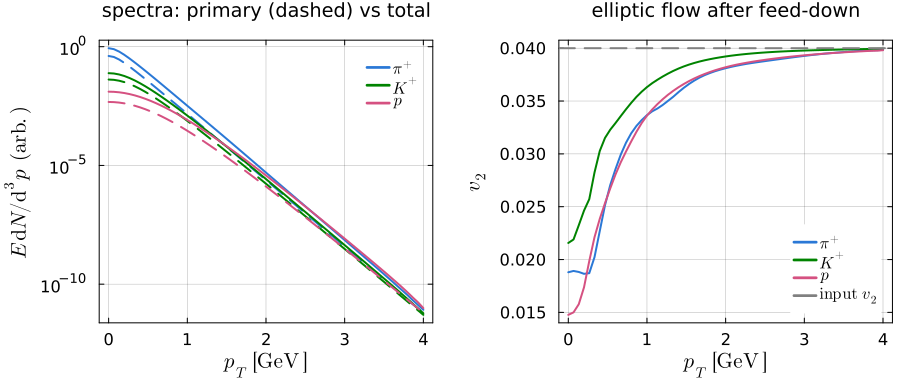
\includegraphics[width=\linewidth]{figures/quickstart.png}
\caption{Full-cascade feed-down for $\pi^+$, $K^+$ and $p$ from a static
thermal source at $T=0.155$~GeV with a flat $4\%$ input $v_2$, computed with
the matrix cascade of Sec.~\ref{sec:cascade}.  \emph{Left:} invariant spectra,
primary component (dashed) against the total after feed-down (solid), on a
logarithmic scale.  \emph{Right:} the resulting $v_2(p_T)$ against the input
value (grey dashed).  Generated by \texttt{quickstart.jl}
$\rightarrow$ \texttt{figures/quickstart.png}.}
\label{fig:quickstart}
\end{figure}

\section{Rapidity-dependent sources: the block-Toeplitz structure}
\label{sec:rapidity}

This section derives the rapidity-dependent extension.  The executable
regression evidence in Sec.~\ref{sec:validation} applies to the currently
implemented \texttt{MassAverage} functor and boost-invariant matrix path; it
does not claim an implementation test of the Toeplitz construction below.

\subsection{The kernel as a rapidity convolution}
\label{sec:conv}

The boost-invariant result of Sec.~\ref{sec:matrix} folded the $\pm\Delta\eta$
contributions together because the source carried no rapidity dependence.
For a general source that fold is not available; instead the rapidity
structure of the kernel must be exposed.  Return to the mode-$n$ decay map
\emph{before} any $\eta$-folding.  The analytic azimuthal integration
[Eq.~(41)] gives, for a rapidity-dependent source,
\begin{equation}
\Fbn(p_T,\eta_p)
=\frac{B\,m_a}{4\pi p_b}
\int_0^\infty\!\mathrm{d}q_T\,q_T
\int_{-\infty}^{\infty}\!\mathrm{d}\Delta\eta\;
\frac{\Theta\!\big(Q^2-D^2\big)}{\sqrt{Q^2-D^2}}\;
2T_n(Z)\;
\Fan\big(q_T,\eta_p+\Delta\eta\big),
\label{eq:etadep-map}
\end{equation}
where the parent rapidity has been written $\eta_q=\eta_p+\Delta\eta$ and
$\mathrm{d}\eta_q=\mathrm{d}\Delta\eta$ at fixed $\eta_p$; every kinematic
quantity $D=M\cosh\Delta\eta-C$, $Z=D/Q$ depends on rapidity only through
$\Delta\eta$.  The daughter rapidity $\eta_p$ therefore appears in
\eqref{eq:etadep-map} \emph{only} as the shift of the source's argument
--- the statement that the decay map commutes with longitudinal boosts,
$\eta_p\to\eta_p+\text{const}$ carrying $\eta_q$ along with it.

Collect everything that multiplies the source into a \emph{profile}
\begin{equation}
K_n(p_T,q_T,\Delta\eta)
\;\equiv\;
\frac{B\,m_a}{4\pi p_b}\,q_T\,
\frac{\Theta\!\big(Q^2-D^2\big)}{\sqrt{Q^2-D^2}}\,
2T_n(Z(q_T,\Delta\eta)),
\label{eq:profile}
\end{equation}
so that \eqref{eq:etadep-map} reads
\begin{equation}
\Fbn(p_T,\eta_p)=\int_0^\infty\!\mathrm{d}q_T
\int_{-\infty}^{\infty}\!\mathrm{d}\Delta\eta\;
K_n(p_T,q_T,\Delta\eta)\;\Fan(q_T,\eta_p+\Delta\eta):
\label{eq:conv}
\end{equation}
at each $(p_T,q_T)$ this is a \emph{convolution} of the source in rapidity
with the fixed profile $K_n(p_T,q_T,\cdot)$.  Three properties of the
profile follow directly from the kernel analysis of Sec.~\ref{sec:window}
and carry the entire structure of what follows:
\begin{enumerate}
\item \textbf{Even:} $K_n(\,\cdot,-\Delta\eta)=K_n(\,\cdot,\Delta\eta)$,
since $D$, $Z$, and $\Theta(Q^2-D^2)$ all depend on $\Delta\eta$ through
$\cosh\Delta\eta$ alone.  The profile is a symmetric rapidity
point-spread function; it does \emph{not} know the sign of the boost.
\item \textbf{Compact support:} $K_n$ vanishes outside
$|\Delta\eta|\in[\eta_{\rm lo},\eta_{\rm hi}]$ (the window of
Sec.~\ref{sec:window}), a set of total rapidity extent
$\le2\,\eta_{\rm hi}=2\operatorname{arccosh}[(C+Q)/M]$, in practice
$1$--$2$ units.
\item \textbf{$\eta_p$-independent:} $K_n$ depends on $p_T$ and $q_T$ but
not on where in rapidity the daughter sits.  This is boost invariance, and
it is what makes \eqref{eq:conv} a genuine convolution rather than a
general integral operator.
\end{enumerate}
Physically $K_n(p_T,q_T,\cdot)$ is the rapidity smearing induced by the
decay: a parent line at a single rapidity feeding daughter momentum
$p_T$ is spread by the profile into a band of daughter rapidities of
width set by $\eta_{\rm hi}$.  A boost-invariant source ($\Fan$
independent of $\eta_q$) is the eigenfunction with the source pulling out
of the convolution, $\Fbn=\big(\int K_n\,\mathrm{d}\Delta\eta\big)\Fan$,
recovering Sec.~\ref{sec:matrix} --- there the $\int K_n\,\mathrm{d}\Delta\eta$
\emph{is} the boost-invariant matrix element.

\subsection{Discretization: the block-Toeplitz matrix}
\label{sec:blocktoeplitz}

Sample both spectra on a common \emph{uniform} rapidity grid
$\eta_a=\eta_0+a\,h_\eta$ (uniformity is essential --- it is what turns the
convolution into a Toeplitz operator).  Index the daughter spectrum by
$(k,a)\leftrightarrow(p_T^{(k)},\eta_a)$ and the parent by
$(j,b)\leftrightarrow(q_T^{(j)},\eta_b)$.  Discretize \eqref{eq:conv} in
two stages.  First the $q_T$ integral and profile, by the same
quadrature-plus-interpolation as Sec.~\ref{sec:matrix}, which produces the
$q_T$ scatter onto column index $j$.  Second the source's rapidity
argument: at a quadrature node with offset $\Delta\eta$, the value
$\Fan(q_T^{(j)},\eta_a+\Delta\eta)$ is reconstructed from the $\eta$ grid
by the uniform Lagrange stencil,
\begin{equation}
\Fan\big(q_T^{(j)},\eta_a+\Delta\eta\big)
\;\approx\;
\sum_{b} L^\eta\!\big(\eta_a+\Delta\eta;\,\eta_b\big)\,
\Fan\big(q_T^{(j)},\eta_b\big).
\end{equation}
The crucial observation is that on a uniform grid the cardinal weight
depends only on the \emph{offset} of the evaluation point from the node in
grid units,
\begin{equation}
L^\eta\big(\eta_a+\Delta\eta;\,\eta_b\big)
=\ell\!\Big(\frac{(\eta_a+\Delta\eta)-\eta_b}{h_\eta}\Big)
=\ell\Big(\frac{\Delta\eta}{h_\eta}-(b-a)\Big),
\label{eq:offsetweight}
\end{equation}
a function of $b-a$ and $\Delta\eta$ but \emph{not} of $a$ and $b$
separately --- translation invariance of the uniform grid, inherited from
translation invariance of the profile.  Assembling the coefficient of
$\Fan(q_T^{(j)},\eta_b)$ in $\Fbn(p_T^{(k)},\eta_a)$ therefore yields a
quantity that depends on the rapidity indices only through $d\equiv b-a$:
\begin{equation}
W\big[(k,a),(j,b)\big]=w\big[k,\,j,\,d\big],
\qquad d=b-a,
\label{eq:toeplitz-index}
\end{equation}
with
\begin{equation}
w[k,j,d]=
\int\!\mathrm{d}\Delta\eta\;\widetilde K_n^{(k,j)}(\Delta\eta)\,
\ell\!\Big(\tfrac{\Delta\eta}{h_\eta}-d\Big),
\label{eq:wtensor}
\end{equation}
$\widetilde K_n^{(k,j)}$ being the profile after the $q_T$
scatter (the quadrature sum over the $q_T$ nodes whose stencil hits column
$j$).  Viewing $W$ as an $N_\eta\times N_\eta$ array of
$N_{p_T}\times N_q$ blocks $B_d=w[\cdot,\cdot,d]$, \eqref{eq:toeplitz-index}
says $W$ is constant along block diagonals,
\begin{equation}
W=
\begin{pmatrix}
B_0 & B_1 & B_2 & \cdots\\
B_{-1} & B_0 & B_1 & \\
B_{-2} & B_{-1} & B_0 & \\
\vdots & & & \ddots
\end{pmatrix},
\end{equation}
a \emph{block-Toeplitz} matrix.  Storing $W$ densely repeats each block up
to $N_\eta$ times; storing the tensor $w[k,j,d]$ once is exact and lossless
--- it is the discrete profile, the point-spread function of
Sec.~\ref{sec:conv} sampled at integer rapidity offsets.

Two further exact properties shrink the tensor, both inherited from the
profile:
\begin{enumerate}
\item \textbf{Banded:} compact support of $K_n$ (item 2 above) plus the
finite reach of the $\eta$ stencil limits the nonzero offsets to
$|d|\le L$ with $L=\lceil\eta_{\rm hi}^{\max}/h_\eta\rceil+\tfrac{P}{2}$
(window half-width plus stencil halo), $\eta_{\rm hi}^{\max}=
\max_{q_T}\operatorname{arccosh}[(C+Q)/M]$, in practice $1$--$2$ units; so
$B_d=0$ for $|d|>L$ and only $2L+1$ offsets exist.
\item \textbf{Even in $d$:} evenness of the profile (item 1) gives
$w[k,j,-d]=w[k,j,d]$, so only $d\ge0$ need be stored.  (The \emph{source}
need not be symmetric in rapidity; the \emph{profile} is.)
\end{enumerate}
For $N_{p_T}=39$, $N_q=121$, $N_\eta=61$, $h_\eta=0.05$,
$L\approx40$: dense $W$ is
$(39\cdot61)\times(121\cdot61)\approx1.76\times10^{7}$ entries
($\sim$140\,MB), the tensor is $39\times121\times41\approx1.9\times10^{5}$
entries ($\sim$1.5\,MB) --- a factor $\sim10^{2}$, at zero accuracy cost,
because it encodes exact symmetries (translation invariance and parity of
the profile) rather than a numerical truncation.

\subsection{Assembly}
\label{sec:toeplitz-assembly}

The assembly generalizes the scatter of Sec.~\ref{sec:matrix} by one
stencil dimension.  Fix a Fourier mode $n$ and run the same
$(q_T,\Delta\eta)$ quadrature loops as the kernel (in $\Delta\eta$ space
--- see the remark below); a node at $(q_T,\Delta\eta)$ with total
quadrature factor
\begin{equation}
\text{fac}
= \text{pref}\cdot v^{q}_i h_q\, q_T\, h_\eta\,
\frac{v^{\theta}_j}{\sqrt{Q^{2}-D^{2}}}\; 2T_n(Z)
\end{equation}
(the $2$ is the two azimuthal roots only --- the $\pm\Delta\eta$ fold is
\emph{not} performed here, each sign now lands on different $\eta$
columns) deposits into the tensor via the product of the $q_T$ stencil
and the $\eta$-offset stencil:
\begin{equation}
w[k,\,j_0+m-1,\,d_0+m'-1] \mathrel{+}= \text{fac}\;
L^{q}_{m}(q_T)\; L^{\eta}_{m'}\!\big(\Delta\eta/h_\eta\big),
\qquad m,m'=1,\dots,P,
\end{equation}
where $d_0$ is the stencil start of the offset $\Delta\eta/h_\eta$ on the
integer offset axis.  Since the kernel factor is even in $\Delta\eta$,
only $\Delta\eta\ge0$ need be traversed and the result stored for
$d\ge0$; the negative offsets are recovered at application time.  No loop
over $\eta_p$ exists anywhere: one sweep per $(k,j)$ column of nodes
builds the profile valid for \emph{every} daughter rapidity, so the
assembly cost equals that of the boost-invariant matrix times the
$P$-fold extra stencil work --- \emph{not} times $N_\eta$.  This is the
payoff of the Toeplitz structure on the assembly side.

Two remarks.  First, the $Z$-space form of Sec.~\ref{sec:zspace} does
\emph{not} apply here: the $\eta$-offset stencil needs the rapidity
$\Delta\eta$ itself, so the assembly stays in $\Delta\eta$ space (or
would have to pay an $\operatorname{arccosh}$ per node to recover
$\Delta\eta$ from $c$ --- exactly the function the $Z$ form eliminates).
Second, the offset variable is interpolated on the \emph{uniform} $\eta$
grid, so the uniform-grid Lagrange weights apply verbatim; the
interpolation error in the $\eta$ direction is the same
$\mathcal O(h_\eta^{P})$ as in $q_T$.

\subsection{Application}

Using the evenness $w[k,j,-d]=w[k,j,d]$, the apply is a folded discrete
convolution over the stored $d\ge0$ half:
\begin{equation}
\Fb\big(p_T^{(k)},\eta_a\big)
=\sum_{j}\Big[\,w[k,j,0]\,\Fa\big(q_T^{(j)},\eta_a\big)
+\sum_{d=1}^{L} w[k,j,d]\,
\big(\Fa\big(q_T^{(j)},\eta_{a+d}\big)+\Fa\big(q_T^{(j)},\eta_{a-d}\big)\big)
\Big].
\label{eq:toeplitz-apply}
\end{equation}
Organizing the computation per offset makes each term a dense
$(N_{p_T}\times N_q)$ matrix acting on an $\eta$-shifted copy of the
source --- $L+1$ small GEMMs over the $(q_T\!\times\!\eta)$ source array:
\begin{equation}
F_b \;=\; \sum_{d=0}^{L} B_d\,\big[S^{+d}F_a + (1-\delta_{d0})\,S^{-d}F_a\big],
\qquad B_d = w[\,\cdot,\cdot,d\,],
\end{equation}
with $S^{\pm d}$ the shift along $\eta$.  Cost:
$\mathcal O(N_{p_T}N_qN_\eta L)$ multiply--adds
($\approx 2\times10^{7}\sim$ milliseconds at
$N_{p_T}{=}39$, $N_q{=}121$, $N_\eta{=}61$, $L{\approx}40$), organized as
BLAS-3 rather than the BLAS-2 of a dense block matrix.  For large
$N_\eta$ the Toeplitz structure admits FFT application along $\eta$,
$\mathcal O(N_{p_T}N_qN_\eta\log N_\eta)$ --- worthwhile only once
$L\gg\log N_\eta$, i.e.\ for very fine rapidity grids; at the sizes above
the direct fold wins.

For azimuthally asymmetric, rapidity-dependent sources the procedure is
per mode as before: one tensor $w_n$ per Fourier mode, assembled with
$2T_n(Z)$, applied to the mode functions $\Fan(q_T,\eta_q)$.

\subsection{Edges and grid layout}

Translation invariance fails only at the ends of the rapidity grid:
daughter points within $\Delta\eta_{\max}$ of the boundary require parent
values beyond it.  Since physical sources vanish rapidly at large $|\eta|$
(e.g.\ $e^{-m_T\cosh\eta/T}$), the consistent convention is zero-padding
--- the same ``source vanishes off the grid'' convention used in $q_T$ ---
with the $\eta$ grid extended by $\Delta\eta_{\max}=
\max_{q_T}\operatorname{arccosh}[(C+Q)/M]$ (evaluated at the band edge;
typically $1$--$2$ units) beyond the rapidity window where results are
needed.  Concretely: to output $|\eta_p|\le\eta^{\rm obs}$, the parent
grid must span $|\eta_q|\lesssim\eta^{\rm obs}+\Delta\eta_{\max}$, and
the truncation error inherits the source's decay at the padding edge ---
for thermal-like sources this is
$e^{-m_{aT}(\cosh(\eta^{\rm obs}+\Delta\eta_{\max})-1)/T}$, negligible
already for modest padding.

The memory layout follows the apply: storing $w$ as
$(k,j)$-major slices per offset $d$ (i.e.\ $L{+}1$ dense
$N_{p_T}\times N_q$ matrices $B_d$) makes each term of
\eqref{eq:toeplitz-apply} a contiguous GEMM; \texttt{Float32} storage is
appropriate for the same reason as in Sec.~\ref{sec:matrix} (rounding
$6\times10^{-8}$, far below the quadrature setting), halving the
$\sim1$--$3$\,MB per decay and mode.

\section{Implementation validation and domain of applicability}
\label{sec:validation}

The results in this section concern the implemented boost-invariant path.
That implementation has two distinct numerical layers.  A
\texttt{MassAverage} evaluates the continuous decay integral directly, while
\texttt{DecayMatrix} or \texttt{decaymatrices} additionally interpolates the
parent spectrum from a finite $q_T$ grid.  A useful validation therefore
checks the integral before checking the matrix: otherwise interpolation and
grid-truncation errors can be mistaken for errors in the decay kernel.

\subsection{Validated operating domain}

For every sharp two-body kernel contained in a two-, three-, or four-body
average, the numerically supported domain is the \emph{strictly open} physical
region
\begin{equation}
 m_a > m_b+\sum_{i\ne b}m_i,\qquad
 m_b>0,\qquad m_i\ge 0 .
 \label{eq:strict-domain}
\end{equation}
The strict inequality matters.  At equality the rest-frame daughter momentum
$p_b$ vanishes.  The two-body prefactor contains $1/p_b$, and the normalization
of a multi-body phase-space average also vanishes.  The limiting decay
distribution can be discussed analytically, but it is not represented by the
fixed-order formulas implemented here.  Branching ratios should be finite and
non-negative, and all quadrature orders
$n_q,n_\theta,n_\mu,n_\sigma,n_{m_a}$ must be positive integers.  The observed
daughter is required to have nonzero mass; a photon may occur among the
unobserved partners, but the present $(p_T,\eta)$ kernel does not return a
massless observed spectrum.

For a finite-width parent the tested Breit--Wigner setup additionally obeys
\begin{equation}
 m_R>0,\qquad \Gamma>0,\qquad
 0<m_{\min}<m_{\max},
 \label{eq:bw-domain}
\end{equation}
normally with $m_{\min}<m_R<m_{\max}$.  The spectral average is normalized on
the full window $[m_{\min},m_{\max}]$, whereas decay-kernel nodes are placed
only in the open portion of that window.  Consequently a channel that is
closed at the pole but open in the high-mass tail retains the correct
open-spectral-weight suppression.

The bundled cascade applies two additional guards before constructing a
matrix: a sharp channel is enrolled only if
$m_a>\sum_i m_i+10^{-6}\,\mathrm{GeV}$, and a broad parent's lower support is
clipped to
\begin{equation}
 m_{\min}=\max(m_R-4\Gamma,\;0.05\,\mathrm{GeV}).
\end{equation}
Thus the exact-threshold and non-positive-support cases discussed below are
excluded by the standard cascade path.  They remain relevant to users calling
the exported decay constructors directly.

\subsection{Independent numerical checks}

For the invariant number functional
\begin{equation}
 {\cal N}[F]=\int_0^\infty q_T\,\mathrm{d}q_T
             \int_{-\infty}^{\infty}\mathrm{d}\eta
             \int_0^{2\pi}\mathrm{d}\phi\,F(q_T,\eta,\phi),
 \label{eq:number-functional}
\end{equation}
an isotropic channel must give ${\cal N}[F_b]=B{\cal N}[F_a]$.  This is a
particularly strong test because it integrates the returned spectrum over the
entire daughter phase space.  The current \texttt{runtests.jl} suite, evaluated
with Julia~1.12.6, gives:
\begin{center}
\begin{tabular}{p{0.34\linewidth}p{0.30\linewidth}p{0.24\linewidth}}
\hline
check & observable & measured result \\
\hline
$\rho\to\pi\pi$, sharp two-body
  & ${\cal N}_b/(B{\cal N}_a)$ & $0.999999$ \\
$\omega\to3\pi$, three-body
  & ${\cal N}_b/(B{\cal N}_a)$ & $1.000069$ \\
$1.3\,\mathrm{GeV}\to4\pi$, four-body
  & ${\cal N}_b/(B{\cal N}_a)$ & $1.000001$ \\
broad $\rho\to\pi\pi$
  & ${\cal N}_b/(B{\cal N}_a)$ & $1.00009$ \\
direct azimuthal result vs.\ $n=0,\pm2$ reconstruction
  & relative difference & at most $10^{-6}$ \\
functor orders doubled
  & two- and three-body relative difference & below $5\times10^{-7}$ \\
\hline
\end{tabular}
\end{center}
These tests use an independent adaptive outer integration of a static
Boltzmann source.  Four-body permutations of the three unobserved cluster
masses also agree within the regression tolerance, checking the nested
Dalitz-area integral rather than merely its normalization.

The sampled matrix is compared separately with the continuous functor.  On
$q_T\in[0,4.2]$ with 121 parent-grid points and fourth-order local Lagrange
interpolation, the maximum relative differences are
\begin{center}
\begin{tabular}{lccc}
\hline
channel and mode & $\rho,\ n=0$ & $\rho,\ n=2$ & $\omega,\ n=0$ \\
\hline
maximum relative difference
 & $2.6\times10^{-5}$ & $2.7\times10^{-4}$ & $3.1\times10^{-5}$ \\
\hline
\end{tabular}
\end{center}
This comparison includes interpolation and the finite parent-grid cutoff; it
is therefore expected to be less precise than the direct quadrature
comparison.  Matrix assembly for the tested modes is deterministic:
\texttt{threaded=true} and \texttt{threaded=false} produce bitwise-identical
matrices.  Negative Fourier indices reuse the even Chebyshev kernel
($W_{-n}=W_n$), and the regression suite also checks non-default integer mode
types such as \texttt{Int8} and \texttt{Int32}.  These results exercise selected
thermal sources and kinematic points; they are regression evidence, not a
proof for every possible input function or grid.

\subsection{Production-order sampled convergence}

The preceding continuous checks use the conservative functor defaults, while
the cascade builds at $(n_q,n_\theta,n_\mu,n_\sigma,n_{m_a})=(32,8,8,8,8)$.
To measure that distinction directly, the bundled list was divided into the
six two-/three-/four-body, sharp/broad strata.  Six reproducibly selected
keys from each stratum were evaluated on the production 134-point
$q_T\in[0,4]$ grid and ten daughter momenta from $0.1$ to $2.0$\,GeV.  The
source was a $T=0.145$\,GeV transverse Boltzmann spectrum with parent
$v_2=0.05$.  Production matrices were compared with
$(128,32,32,32,32)$ matrices of the same grid and interpolation order.

For mode zero, let $\epsilon_0$ be the maximum absolute spectrum difference
normalized by the reference peak.  For mode two, a relative error can become
arbitrarily large when the true response crosses zero, so the physical metric
is instead the maximum absolute error in the daughter
$v_2=F_2/F_0$:
\begin{center}\small
\begin{tabular}{lrrrr}
\hline
key stratum
& median $\epsilon_0$ & max.\ $\epsilon_0$
& median $|\Delta v_2|$ & max.\ $|\Delta v_2|$\\
\hline
two-body, sharp   & $1.05{\times}10^{-4}$ & $1.81{\times}10^{-4}$ & $8.35{\times}10^{-6}$ & $1.39{\times}10^{-5}$\\
two-body, broad   & $5.81{\times}10^{-4}$ & $8.66{\times}10^{-3}$ & $8.28{\times}10^{-4}$ & $2.77{\times}10^{-3}$\\
three-body, sharp & $2.43{\times}10^{-3}$ & $2.39{\times}10^{-2}$ & $1.63{\times}10^{-3}$ & $7.27{\times}10^{-3}$\\
three-body, broad & $4.02{\times}10^{-3}$ & $1.37{\times}10^{-2}$ & $1.93{\times}10^{-3}$ & $4.66{\times}10^{-3}$\\
four-body, sharp  & $2.62{\times}10^{-2}$ & $9.50{\times}10^{-2}$ & $9.14{\times}10^{-3}$ & $1.43{\times}10^{-2}$\\
four-body, broad  & $1.25{\times}10^{-2}$ & $2.22{\times}10^{-2}$ & $4.46{\times}10^{-3}$ & $7.11{\times}10^{-3}$\\
\hline
\end{tabular}
\end{center}
These are small per-stratum samples, not a population-weighted full-cascade
error bar.  Nevertheless,
checking the worst sampled key in each stratum against
$(256,64,64,64,64)$ left only $2.4\,10^{-6}$--$8.8\,10^{-6}$ residual
mode-zero error and at most $5.2\,10^{-4}$ residual absolute $v_2$ error, so
the observed production-order differences are not reference noise.

Rounding each matrix to \texttt{Float32} is not the limitation: over all 72
sampled key--mode applications its median effect was $5.9\,10^{-9}$ and its
maximum was $2.5\,10^{-8}$.  The convergence study instead isolates
$n_\mu=8$ as the main three-/four-body limitation and $n_{m_a}=8$ as the
additional broad-parent limitation; increasing $n_q$, $n_\theta$, or
$n_\sigma$ alone had little effect in the difficult sampled cases.

A selective candidate
$(n_q,n_\theta,n_\mu,n_\sigma,n_{m_a})=(32,8,16,8,16)$ was checked on the
worst sampled mode-zero key of every stratum.  The largest mode-zero error
fell from $9.50\,10^{-2}$ to $8.51\,10^{-4}$, and the largest absolute
daughter-$v_2$ error fell from $1.39\,10^{-2}$ to $3.38\,10^{-3}$.
This changes only one-time construction work; matrix size and cascade-apply
speed are unchanged.  It is therefore the first accuracy setting to try when
multi-body anisotropy matters, followed by an order-doubling check for the
specific observables.

There is still no single independently measured ``full-cascade percentage'':
the answer depends on branching ratios, the primary spectra, cancellations,
and how errors propagate through successive generations.  The current
cascade-vs-direct regression uses the same low-order kernels on both sides,
so it validates branching ratios, multiplicity, ordering, persistence, and
\texttt{Float32} wiring rather than production quadrature accuracy.  A
high-order end-to-end cascade comparison remains desirable.

\subsection{Finite-width threshold stress test}

The difficult finite-width case is a narrow open sliver: the pole lies below
threshold and only the upper end of the spectral window can decay.  Sampling
the whole window with ordinary nodes and discarding closed nodes can miss this
sliver completely.  The implementation instead splits the parent-mass
quadrature at threshold and places all decay nodes in the open interval.  For
the deliberately severe test
\begin{equation}
 [m_{\min},m_{\max}]=[0.6,1.4]\,\mathrm{GeV},\qquad
 m_{\mathrm{threshold}}=1.3\,\mathrm{GeV},
\end{equation}
\texttt{nma=8} gives a nonzero matrix.  Relative to an
\texttt{nma=96} reference, the integrated matrix deviation decreases from
approximately $0.15$ at \texttt{nma=8} to $0.04$ at \texttt{nma=32}.
Therefore threshold splitting fixes the silent-zero failure, but does not make
a very small open fraction cheap to resolve.  For custom decay lists with such
channels, \texttt{nma} should be increased until the result is stable; the
default is intended for ordinary, well-open windows.  The bundled decay list
currently enrolls no tail-reopened channels; the stress case is retained to
protect custom lists and future data updates.

\subsection{Known boundary behavior and recommended safeguards}

Two classes of input are rejected by the library itself, at construction.
The sharp constructors test openness strictly, so exact equality in
\eqref{eq:strict-domain} raises rather than producing an infinite two-body
coefficient or a \texttt{NaN} three- or four-body normalization; and
\texttt{BreitWigner} requires finite arguments with $m_R>0$, $\Gamma>0$ and
$0\le m_{\min}<m_{\max}$, as in \eqref{eq:bw-domain}, while the five quadrature
orders are required to be at least one.  These guards are not cosmetic: a
non-positive width, a non-positive pole mass or a reversed interval each
yields an \emph{empty} parent-mass average --- a channel whose matrix is
identically zero, which feeds nothing downstream and reports nothing --- and a
negative width inverts the support interval on its own.  The keyword form
still clamps a negative $m_{\min}$ to zero, which is a legitimate
case: fourteen states in the QM2016 list are broad enough for the default
$m_R-k\Gamma$ to fall below zero.

The following remain outside the validated domain and must be handled by the
calling application:
\begin{enumerate}
\item The arrays inside \texttt{MassAverage} --- its node lists, and the
quadrature rules reached through \texttt{kern} --- are treated as immutable by
the library and are shared between every channel built from the same
\texttt{Rules}.  Sharing makes them safe for concurrent reads, and they are
built eagerly before any task starts, so no reader can observe a partial one;
but the objects are exported, and user code must not mutate them.  Mutating one
would corrupt every channel that shares it, not only the channel at hand.
\item For a broad channel whose open part is only a small fraction of its
support, convergence in \texttt{nma} must be checked separately from
convergence in $n_q,n_\theta,n_\mu,n_\sigma$.  Increasing the kernel orders
cannot repair an under-resolved parent-mass average.
\item A matrix represents the parent source only on its supplied $q_T$ grid.
The interpolation convention is zero outside that grid, so its upper endpoint
must be placed where the omitted parent tail is negligible.  This is a matrix
domain choice, not an error of the continuous decay functor.
\end{enumerate}

Of the checks a robust production setup needs, the library performs those
it can state locally: masses against the strict threshold, widths and support
bounds through \texttt{BreitWigner}, the quadrature orders, and the rejection
of any non-finite coefficient arising from a near-threshold node of a broad
parent.  What it cannot check is what only the caller knows --- that the
branching ratios are the intended ones, that the $q_T$ grid extends past the
parent tail, and that \texttt{nma} has been converged separately for a narrowly
reopened channel.  Number conservation and matrix--functor agreement should be
kept as regression tests regardless.  None of this touches the fast path: once
valid matrices have been built, feed-down remains a sequence of in-place
matrix--vector products.

\section{Summary}

\begin{center}
\begin{tabular}{
>{\raggedright\arraybackslash}p{0.21\linewidth}
>{\raggedright\arraybackslash}p{0.29\linewidth}
>{\raggedright\arraybackslash}p{0.38\linewidth}}
\hline
case & object & size / cost \\
\hline
$\eta$-independent, per mode $n$ & logical dense operator $W_n$ with
row-band cascade storage &
$\sim$38\,KiB for $39\times121$ \texttt{Float64}
($\sim$70\,KiB for $134^2$ \texttt{Float32}); apply $\sim\mu$s \\
full cascade, current defaults & $18{,}299$ keys, two modes on $134^2$ &
$2.4481$\,GiB dense baseline; $1.1012$\,GiB estimated packed payload
($44.98\%$); production full-apply timing pending \\
$\eta$-dependent, per mode $n$ & tensor $w[k,j,d]$, $|d|\le L$, $d\ge0$ &
$\sim$0.8\,MiB for $39\times121\times41$ \texttt{Float32}; apply $\sim$ms \\
\hline
\end{tabular}
\end{center}

\end{document}
